%%=============================================================================
%% LaTeX sjabloon voor bachelorproef, HoGent Bedrijf en Organisatie
%% Opleiding Toegepaste Informatica
%%=============================================================================

\documentclass[fleqn,a4paper,12pt]{book}

%%=============================================================================
%% LaTeX sjabloon voor de bachelorproef, HoGent Bedrijf en Organisatie
%% Opleiding toegepaste informatica
%%
%% Structuur en algemene vormgeving. Meestal hoef je hier niets te wijzigen.
%%
%% Vormgeving gebaseerd op "The Legrand Orange Book", version 2.0 (9/2/15)
%% door Mathias Legrand (legrand.mathias@gmail.com) met aanpassingen door
%% Vel (vel@latextemplates.com). Het oorspronkelijke template is te vinden op
%% http://www.LaTeXTemplates.com
%%
%% Aanpassingen voor HoGent toegepaste informatica: 
%%   Bert Van Vreckem <bert.vanvreckem@hogent.be>
%% Licentie: 
%%   CC BY-NC-SA 3.0 (http://creativecommons.org/licenses/by-nc-sa/3.0/)
%%=============================================================================
%%--------------- glossary



% eigen aangemaakt
\usepackage{longtable}
\usepackage[acronym]{glossaries}
\usepackage{makecell}
\usepackage{wrapfig}
\usepackage{listings}  
\usepackage[final]{pdfpages}
\usepackage{scrextend}
\usepackage{listings} %For code in appendix
\lstset
{ %Formatting for code in appendix
    language=Matlab,
    basicstyle=\footnotesize,
    numbers=left,
    stepnumber=1,
    showstringspaces=false,
    tabsize=1,
    breaklines=true,
    breakatwhitespace=false,
}

\usepackage{mathtools}

% -------------------------------------------------------glossary

\makeglossaries
%%----------------

%%-----------------------------------------------------------------------------
%% Packages
%%-----------------------------------------------------------------------------

\usepackage[top=3cm,bottom=3cm,left=3cm,right=3cm,headsep=10pt,a4paper]{geometry} % Page margins
\usepackage[utf8]{inputenc}  % Accenten gebruiken in tekst (vb. é ipv \'e)
\usepackage{amsfonts}        % AMS math packages: extra wiskundige
\usepackage{amsmath}         %   symbolen (o.a. getallen-
\usepackage{amssymb}         %   verzamelingen N, R, Z, Q, etc.)
\usepackage[english,dutch]{babel}    % Taalinstellingen: woordsplitsingen,
                             %  commando's voor speciale karakters
                             %  ("dutch" voor NL)
\usepackage{iflang}
\usepackage{eurosym}         % Euro-symbool €
\usepackage{geometry}
\usepackage{graphicx}        % Invoegen van tekeningen
\graphicspath{{img/}}       % Specifies the directory where pictures are stored
\usepackage{tikz}            % Required for drawing custom shapes
\usepackage[pdftex,bookmarks=true]{hyperref}
                             % PDF krijgt klikbare links & verwijzingen,
                             %  inhoudstafel
\usepackage{enumitem}        % Customize lists
\setlist{nolistsep}         % Reduce spacing between list items
\usepackage{listings}        % Broncode mooi opmaken
\usepackage{multirow}        % Tekst over verschillende cellen in tabellen
\usepackage{rotating}        % Tabellen en figuren roteren

\usepackage{booktabs}        % Required for nicer horizontal rules in tables

\usepackage{xcolor}          % Required for specifying colors by name
\definecolor{maincolor}{RGB}{0,147,208} % Define the main color used for 
                             % highlighting throughout the book
                             % 0, 147, 208 = officiële kleur HoGent FBO

% Paragraph style: no indent, add space between paragraphs
\setlength{\parindent}{0em}
\setlength{\parskip}{1em}

\usepackage{etoolbox}
\usepackage{titling} % Macros for title, author, etc
\usepackage{lipsum}          % Voor vultekst (lorem ipsum)

%----------------------------------------------------------------------------------------
%	FONTS
%----------------------------------------------------------------------------------------

\usepackage{avant} % Use the Avantgarde font for headings
%\usepackage{times} % Use the Times font for headings
\usepackage{mathptmx} % Use the Adobe Times Roman as the default text font together with math symbols from the Sym­bol, Chancery and Com­puter Modern fonts

\usepackage{microtype} % Slightly tweak font spacing for aesthetics
\usepackage[utf8]{inputenc} % Required for including letters with accents
\usepackage[T1]{fontenc} % Use 8-bit encoding that has 256 glyphs

%------------------------------------------------------------------------------
%	TITLE PAGE
%------------------------------------------------------------------------------

\newcommand{\inserttitlepage}{%
\begin{titlepage}
  \newgeometry{top=2cm,bottom=1.5cm,left=1.5cm,right=1.5cm}
  \begin{center}

    \begingroup
    \rmfamily
    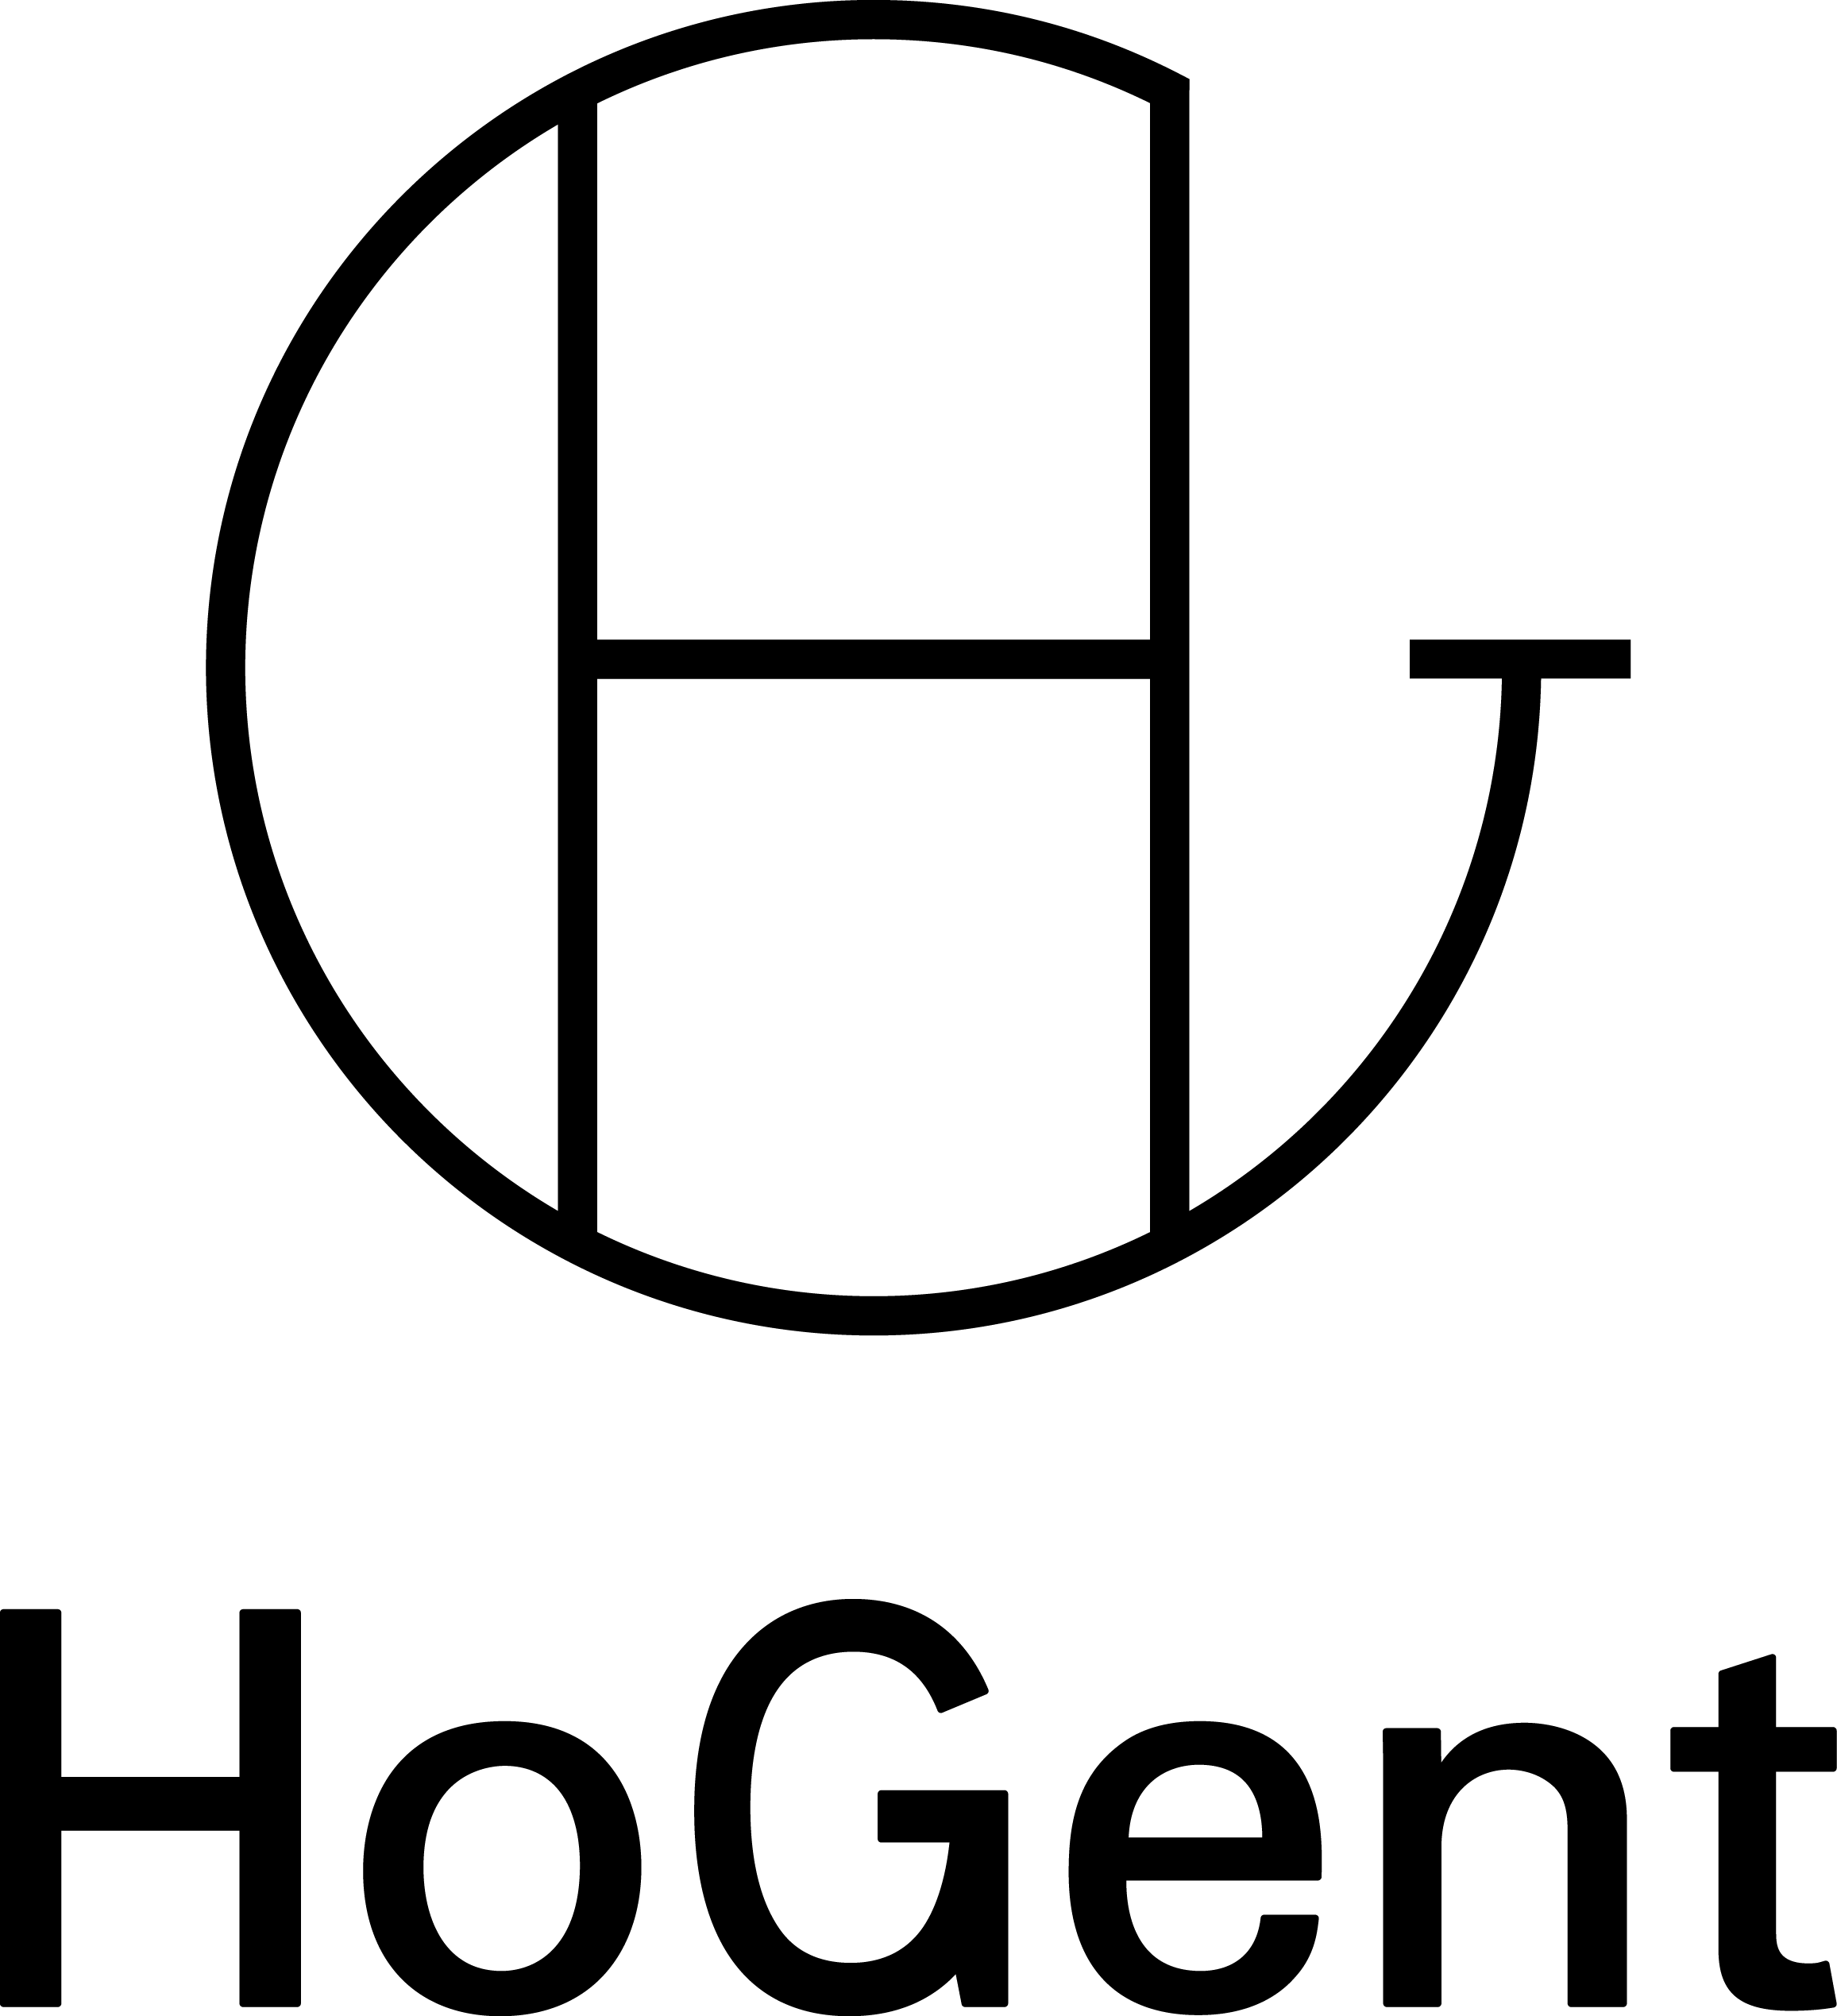
\includegraphics[width=2.5cm]{img/HG-beeldmerk-woordmerk}\\[.5cm]
    Faculteit Bedrijf en Organisatie\\[3cm]
    \titel
    \vfill
    \student\\[3.5cm]
    Scriptie voorgedragen tot het bekomen van de graad van\\professionele bachelor in de toegepaste informatica\\[2cm]
    Promotor:\\
    \promotor\\
    \ifdefempty{\copromotor}{\vspace{2.5cm}}{Co-promotor:\\\copromotor\\[2.5cm]}
    Instelling: \instelling\\[.5cm]
    Academiejaar: \academiejaar\\[.5cm]
    \ifcase \examenperiode \or Eerste \or Tweede \else Derde \fi examenperiode
    \endgroup

  \end{center}
  \restoregeometry
\end{titlepage}
  \emptypage
\begin{titlepage}
  \newgeometry{top=5.35cm,bottom=1.5cm,left=1.5cm,right=1.5cm}
  \begin{center}

    \begingroup
    \rmfamily
    \IfLanguageName{dutch}{Faculteit Bedrijf en Organisatie}{Faculty of Business and Information Management}\\[3cm]
    \titel
    \vfill
    \student\\[3.5cm]
    \IfLanguageName{dutch}{Scriptie voorgedragen tot het bekomen van de graad van\\professionele bachelor in de toegepaste informatica}{Thesis submitted in partial fulfillment of the requirements for the degree of\\professional bachelor of applied computer science}\\[2cm]
    Promotor:\\
    \promotor\\
    \ifdefempty{\copromotor}{\vspace{2.5cm}}{Co-promotor:\\\copromotor\\[2.5cm]}
    \IfLanguageName{dutch}{Instelling}{Institution}: \instelling\\[.5cm]
    \IfLanguageName{dutch}{Academiejaar}{Academic year}: \academiejaar\\[.5cm]
    \IfLanguageName{dutch}{%
    \ifcase \examenperiode \or Eerste \or Tweede \else Derde \fi examenperiode}{%
    \ifcase \examenperiode \or First \or Second \else Third \fi examination period}
    \endgroup

  \end{center}
  \restoregeometry
\end{titlepage}
}

%----------------------------------------------------------------------------------------
%	BIBLIOGRAPHY AND INDEX
%----------------------------------------------------------------------------------------

\usepackage[style=apa,backend=biber]{biblatex}
\usepackage{csquotes}
\DeclareLanguageMapping{dutch}{dutch-apa}
\addbibresource{bachproef-tin.bib} % BibTeX bibliography file
\defbibheading{bibempty}{}

\usepackage{calc} % For simpler calculation - used for spacing the index letter headings correctly
\usepackage{makeidx} % Required to make an index
\makeindex % Tells LaTeX to create the files required for indexing

%----------------------------------------------------------------------------------------
%	MAIN TABLE OF CONTENTS
%----------------------------------------------------------------------------------------

\usepackage{titletoc} % Required for manipulating the table of contents

\contentsmargin{0cm} % Removes the default margin

% Part text styling
\titlecontents{part}[0cm]
{\addvspace{20pt}\centering\large\bfseries}
{}
{}
{}

% Chapter text styling
\titlecontents{chapter}[1.25cm] % Indentation
{\addvspace{12pt}\large\sffamily\bfseries} % Spacing and font options for chapters
{\color{maincolor!60}\contentslabel[\Large\thecontentslabel]{1.25cm}\color{maincolor}} % Chapter number
{\color{maincolor}}
{\color{maincolor!60}\normalsize\;\titlerule*[.5pc]{.}\;\thecontentspage} % Page number

% Section text styling
\titlecontents{section}[1.25cm] % Indentation
{\addvspace{3pt}\sffamily\bfseries} % Spacing and font options for sections
{\contentslabel[\thecontentslabel]{1.25cm}} % Section number
{}
{\hfill\color{black}\thecontentspage} % Page number
[]

% Subsection text styling
\titlecontents{subsection}[1.25cm] % Indentation
{\addvspace{1pt}\sffamily\small} % Spacing and font options for subsections
{\contentslabel[\thecontentslabel]{1.25cm}} % Subsection number
{}
{\ \titlerule*[.5pc]{.}\;\thecontentspage} % Page number
[]

% List of figures
\titlecontents{figure}[0em]
{\addvspace{-5pt}\sffamily}
{\thecontentslabel\hspace*{1em}}
{}
{\ \titlerule*[.5pc]{.}\;\thecontentspage}
[]

% List of tables
\titlecontents{table}[0em]
{\addvspace{-5pt}\sffamily}
{\thecontentslabel\hspace*{1em}}
{}
{\ \titlerule*[.5pc]{.}\;\thecontentspage}
[]

%----------------------------------------------------------------------------------------
%	MINI TABLE OF CONTENTS IN PART HEADS
%----------------------------------------------------------------------------------------

% Chapter text styling
\titlecontents{lchapter}[0em] % Indenting
{\addvspace{15pt}\large\sffamily\bfseries} % Spacing and font options for chapters
{\color{maincolor}\contentslabel[\Large\thecontentslabel]{1.25cm}\color{maincolor}} % Chapter number
{}
{\color{maincolor}\normalsize\sffamily\bfseries\;\titlerule*[.5pc]{.}\;\thecontentspage} % Page number

% Section text styling
\titlecontents{lsection}[0em] % Indenting
{\sffamily\small} % Spacing and font options for sections
{\contentslabel[\thecontentslabel]{1.25cm}} % Section number
{}
{}

% Subsection text styling
\titlecontents{lsubsection}[.5em] % Indentation
{\normalfont\footnotesize\sffamily} % Font settings
{}
{}
{}

%----------------------------------------------------------------------------------------
%	PAGE HEADERS
%----------------------------------------------------------------------------------------

\usepackage{fancyhdr} % Required for header and footer configuration

\pagestyle{fancy}
\renewcommand{\chaptermark}[1]{\markboth{\sffamily\normalsize\bfseries\chaptername\ \thechapter.\ #1}{}} % Chapter text font settings
\renewcommand{\sectionmark}[1]{\markright{\sffamily\normalsize\thesection\hspace{5pt}#1}{}} % Section text font settings
\fancyhf{} \fancyhead[LE,RO]{\sffamily\normalsize\thepage} % Font setting for the page number in the header
\fancyhead[LO]{\rightmark} % Print the nearest section name on the left side of odd pages
\fancyhead[RE]{\leftmark} % Print the current chapter name on the right side of even pages
\renewcommand{\headrulewidth}{0.5pt} % Width of the rule under the header
\addtolength{\headheight}{2.5pt} % Increase the spacing around the header slightly
\renewcommand{\footrulewidth}{0pt} % Removes the rule in the footer
\fancypagestyle{plain}{\fancyhead{}\renewcommand{\headrulewidth}{0pt}} % Style for when a plain pagestyle is specified

% Removes the header from odd empty pages at the end of chapters
\makeatletter
\renewcommand{\cleardoublepage}{
\clearpage\ifodd\c@page\else
\hbox{}
\vspace*{\fill}
\thispagestyle{empty}
\newpage
\fi}

%----------------------------------------------------------------------------------------
%	THEOREM STYLES
%----------------------------------------------------------------------------------------

\usepackage{amsmath,amsfonts,amssymb,amsthm} % For math equations, theorems, symbols, etc

\newcommand{\intoo}[2]{\mathopen{]}#1\,;#2\mathclose{[}}
\newcommand{\ud}{\mathop{\mathrm{{}d}}\mathopen{}}
\newcommand{\intff}[2]{\mathopen{[}#1\,;#2\mathclose{]}}
\newtheorem{notation}{Notation}[chapter]

% Boxed/framed environments
\newtheoremstyle{maincolornumbox}% % Theorem style name
{0pt}% Space above
{0pt}% Space below
{\normalfont}% % Body font
{}% Indent amount
{\small\bf\sffamily\color{maincolor}}% % Theorem head font
{\;}% Punctuation after theorem head
{0.25em}% Space after theorem head
{\small\sffamily\color{maincolor}\thmname{#1}\nobreakspace\thmnumber{\@ifnotempty{#1}{}\@upn{#2}}% Theorem text (e.g. Theorem 2.1)
\thmnote{\nobreakspace\the\thm@notefont\sffamily\bfseries\color{black}---\nobreakspace#3.}} % Optional theorem note
\renewcommand{\qedsymbol}{$\blacksquare$}% Optional qed square

\newtheoremstyle{blacknumex}% Theorem style name
{5pt}% Space above
{5pt}% Space below
{\normalfont}% Body font
{} % Indent amount
{\small\bf\sffamily}% Theorem head font
{\;}% Punctuation after theorem head
{0.25em}% Space after theorem head
{\small\sffamily{\tiny\ensuremath{\blacksquare}}\nobreakspace\thmname{#1}\nobreakspace\thmnumber{\@ifnotempty{#1}{}\@upn{#2}}% Theorem text (e.g. Theorem 2.1)
\thmnote{\nobreakspace\the\thm@notefont\sffamily\bfseries---\nobreakspace#3.}}% Optional theorem note

\newtheoremstyle{blacknumbox} % Theorem style name
{0pt}% Space above
{0pt}% Space below
{\normalfont}% Body font
{}% Indent amount
{\small\bf\sffamily}% Theorem head font
{\;}% Punctuation after theorem head
{0.25em}% Space after theorem head
{\small\sffamily\thmname{#1}\nobreakspace\thmnumber{\@ifnotempty{#1}{}\@upn{#2}}% Theorem text (e.g. Theorem 2.1)
\thmnote{\nobreakspace\the\thm@notefont\sffamily\bfseries---\nobreakspace#3.}}% Optional theorem note

% Non-boxed/non-framed environments
\newtheoremstyle{maincolornum}% % Theorem style name
{5pt}% Space above
{5pt}% Space below
{\normalfont}% % Body font
{}% Indent amount
{\small\bf\sffamily\color{maincolor}}% % Theorem head font
{\;}% Punctuation after theorem head
{0.25em}% Space after theorem head
{\small\sffamily\color{maincolor}\thmname{#1}\nobreakspace\thmnumber{\@ifnotempty{#1}{}\@upn{#2}}% Theorem text (e.g. Theorem 2.1)
\thmnote{\nobreakspace\the\thm@notefont\sffamily\bfseries\color{black}---\nobreakspace#3.}} % Optional theorem note
\renewcommand{\qedsymbol}{$\blacksquare$}% Optional qed square
\makeatother

% Defines the theorem text style for each type of theorem to one of the three styles above
\newcounter{dummy}
\numberwithin{dummy}{section}
\theoremstyle{maincolornumbox}
\newtheorem{theoremeT}[dummy]{Theorem}
\newtheorem{problem}{Problem}[chapter]
\newtheorem{exerciseT}{Exercise}[chapter]
\theoremstyle{blacknumex}
\newtheorem{exampleT}{Example}[chapter]
\theoremstyle{blacknumbox}
\newtheorem{vocabulary}{Vocabulary}[chapter]
\newtheorem{definitionT}{Definition}[section]
\newtheorem{corollaryT}[dummy]{Corollary}
\theoremstyle{maincolornum}
\newtheorem{proposition}[dummy]{Proposition}

%----------------------------------------------------------------------------------------
%	DEFINITION OF COLORED BOXES
%----------------------------------------------------------------------------------------

\RequirePackage[framemethod=default]{mdframed} % Required for creating the theorem, definition, exercise and corollary boxes

% Theorem box
\newmdenv[skipabove=7pt,
skipbelow=7pt,
backgroundcolor=black!5,
linecolor=maincolor,
innerleftmargin=5pt,
innerrightmargin=5pt,
innertopmargin=5pt,
leftmargin=0cm,
rightmargin=0cm,
innerbottommargin=5pt]{tBox}

% Exercise box
\newmdenv[skipabove=7pt,
skipbelow=7pt,
rightline=false,
leftline=true,
topline=false,
bottomline=false,
backgroundcolor=maincolor!10,
linecolor=maincolor,
innerleftmargin=5pt,
innerrightmargin=5pt,
innertopmargin=5pt,
innerbottommargin=5pt,
leftmargin=0cm,
rightmargin=0cm,
linewidth=4pt]{eBox}

% Definition box
\newmdenv[skipabove=7pt,
skipbelow=7pt,
rightline=false,
leftline=true,
topline=false,
bottomline=false,
linecolor=maincolor,
innerleftmargin=5pt,
innerrightmargin=5pt,
innertopmargin=0pt,
leftmargin=0cm,
rightmargin=0cm,
linewidth=4pt,
innerbottommargin=0pt]{dBox}

% Corollary box
\newmdenv[skipabove=7pt,
skipbelow=7pt,
rightline=false,
leftline=true,
topline=false,
bottomline=false,
linecolor=gray,
backgroundcolor=black!5,
innerleftmargin=5pt,
innerrightmargin=5pt,
innertopmargin=5pt,
leftmargin=0cm,
rightmargin=0cm,
linewidth=4pt,
innerbottommargin=5pt]{cBox}

% Creates an environment for each type of theorem and assigns it a theorem text style from the "Theorem Styles" section above and a colored box from above
\newenvironment{theorem}{\begin{tBox}\begin{theoremeT}}{\end{theoremeT}\end{tBox}}
\newenvironment{exercise}{\begin{eBox}\begin{exerciseT}}{\hfill{\color{maincolor}\tiny\ensuremath{\blacksquare}}\end{exerciseT}\end{eBox}}
\newenvironment{definition}{\begin{dBox}\begin{definitionT}}{\end{definitionT}\end{dBox}}
\newenvironment{example}{\begin{exampleT}}{\hfill{\tiny\ensuremath{\blacksquare}}\end{exampleT}}
\newenvironment{corollary}{\begin{cBox}\begin{corollaryT}}{\end{corollaryT}\end{cBox}}

%----------------------------------------------------------------------------------------
%	REMARK ENVIRONMENT
%----------------------------------------------------------------------------------------

\newenvironment{remark}{\par\vspace{10pt}\small % Vertical white space above the remark and smaller font size
\begin{list}{}{
\leftmargin=35pt % Indentation on the left
\rightmargin=25pt}\item\ignorespaces % Indentation on the right
\makebox[-2.5pt]{\begin{tikzpicture}[overlay]
\node[draw=maincolor!60,line width=1pt,circle,fill=maincolor!25,font=\sffamily\bfseries,inner sep=2pt,outer sep=0pt] at (-15pt,0pt){\textcolor{maincolor}{R}};\end{tikzpicture}} % Orange R in a circle
\advance\baselineskip -1pt}{\end{list}\vskip5pt} % Tighter line spacing and white space after remark

%----------------------------------------------------------------------------------------
%	SECTION NUMBERING IN THE MARGIN
%----------------------------------------------------------------------------------------

\makeatletter
\renewcommand{\@seccntformat}[1]{\llap{\textcolor{maincolor}{\csname the#1\endcsname}\hspace{1em}}}
\renewcommand{\section}{\@startsection{section}{1}{\z@}
{-4ex \@plus -1ex \@minus -.4ex}
{1ex \@plus.2ex }
{\normalfont\large\sffamily\bfseries}}
\renewcommand{\subsection}{\@startsection {subsection}{2}{\z@}
{-3ex \@plus -0.1ex \@minus -.4ex}
{0.5ex \@plus.2ex }
{\normalfont\sffamily\bfseries}}
\renewcommand{\subsubsection}{\@startsection {subsubsection}{3}{\z@}
{-2ex \@plus -0.1ex \@minus -.2ex}
{.2ex \@plus.2ex }
{\normalfont\small\sffamily\bfseries}}
\renewcommand\paragraph{\@startsection{paragraph}{4}{\z@}
{-2ex \@plus-.2ex \@minus .2ex}
{.1ex}
{\normalfont\small\sffamily\bfseries}}

%----------------------------------------------------------------------------------------
%	PART HEADINGS
%----------------------------------------------------------------------------------------

% numbered part in the table of contents
\newcommand{\@mypartnumtocformat}[2]{%
\setlength\fboxsep{0pt}%
\noindent\colorbox{maincolor!20}{\strut\parbox[c][.7cm]{\ecart}{\color{maincolor!70}\Large\sffamily\bfseries\centering#1}}\hskip\esp\colorbox{maincolor!40}{\strut\parbox[c][.7cm]{\linewidth-\ecart-\esp}{\Large\sffamily\centering#2}}}%
%%%%%%%%%%%%%%%%%%%%%%%%%%%%%%%%%%
% unnumbered part in the table of contents
\newcommand{\@myparttocformat}[1]{%
\setlength\fboxsep{0pt}%
\noindent\colorbox{maincolor!40}{\strut\parbox[c][.7cm]{\linewidth}{\Large\sffamily\centering#1}}}%
%%%%%%%%%%%%%%%%%%%%%%%%%%%%%%%%%%
\newlength\esp
\setlength\esp{4pt}
\newlength\ecart
\setlength\ecart{1.2cm-\esp}
\newcommand{\thepartimage}{}%
\newcommand{\partimage}[1]{\renewcommand{\thepartimage}{#1}}%
\def\@part[#1]#2{%
\ifnum \c@secnumdepth >-2\relax%
\refstepcounter{part}%
\addcontentsline{toc}{part}{\texorpdfstring{\protect\@mypartnumtocformat{\thepart}{#1}}{\partname~\thepart\ ---\ #1}}
\else%
\addcontentsline{toc}{part}{\texorpdfstring{\protect\@myparttocformat{#1}}{#1}}%
\fi%
\startcontents%
\markboth{}{}%
{\thispagestyle{empty}%
\begin{tikzpicture}[remember picture,overlay]%
\node at (current page.north west){\begin{tikzpicture}[remember picture,overlay]%
\fill[maincolor!20](0cm,0cm) rectangle (\paperwidth,-\paperheight);
\node[anchor=north] at (4cm,-3.25cm){\color{maincolor!40}\fontsize{220}{100}\sffamily\bfseries\@Roman\c@part};
\node[anchor=south east] at (\paperwidth-1cm,-\paperheight+1cm){\parbox[t][][t]{8.5cm}{
\printcontents{l}{0}{\setcounter{tocdepth}{1}}%
}};
\node[anchor=north east] at (\paperwidth-1.5cm,-3.25cm){\parbox[t][][t]{15cm}{\strut\raggedleft\color{white}\fontsize{30}{30}\sffamily\bfseries#2}};
\end{tikzpicture}};
\end{tikzpicture}}%
\@endpart}
\def\@spart#1{%
\startcontents%
\phantomsection
{\thispagestyle{empty}%
\begin{tikzpicture}[remember picture,overlay]%
\node at (current page.north west){\begin{tikzpicture}[remember picture,overlay]%
\fill[maincolor!20](0cm,0cm) rectangle (\paperwidth,-\paperheight);
\node[anchor=north east] at (\paperwidth-1.5cm,-3.25cm){\parbox[t][][t]{15cm}{\strut\raggedleft\color{white}\fontsize{30}{30}\sffamily\bfseries#1}};
\end{tikzpicture}};
\end{tikzpicture}}
\addcontentsline{toc}{part}{\texorpdfstring{%
\setlength\fboxsep{0pt}%
\noindent\protect\colorbox{maincolor!40}{\strut\protect\parbox[c][.7cm]{\linewidth}{\Large\sffamily\protect\centering #1\quad\mbox{}}}}{#1}}%
\@endpart}
\def\@endpart{\vfil\newpage
\if@twoside
\if@openright
\null
\thispagestyle{empty}%
\newpage
\fi
\fi
\if@tempswa
\twocolumn
\fi}

%----------------------------------------------------------------------------------------
%	CHAPTER HEADINGS
%----------------------------------------------------------------------------------------

% A switch to conditionally include a picture, implemented by  Christian Hupfer
\newif\ifusechapterimage
\usechapterimagetrue
\newcommand{\thechapterimage}{}%
\newcommand{\chapterimage}[1]{\ifusechapterimage\renewcommand{\thechapterimage}{#1}\fi}%
\def\@makechapterhead#1{%
{\parindent \z@ \raggedright \normalfont
\ifnum \c@secnumdepth >\m@ne
\if@mainmatter
\begin{tikzpicture}[remember picture,overlay]
\node at (current page.north west)
{\begin{tikzpicture}[remember picture,overlay]
\node[anchor=north west,inner sep=0pt] at (0,0) {\ifusechapterimage\includegraphics[width=\paperwidth]{\thechapterimage}\fi};
\draw[anchor=west] (\Gm@lmargin,-9cm) node [line width=2pt,rounded corners=15pt,draw=maincolor,fill=white,fill opacity=0.5,inner sep=15pt]{\strut\makebox[22cm]{}};
\draw[anchor=west] (\Gm@lmargin+.3cm,-9cm) node {\huge\sffamily\bfseries\color{black}\thechapter. #1\strut};
\end{tikzpicture}};
\end{tikzpicture}
\else
\begin{tikzpicture}[remember picture,overlay]
\node at (current page.north west)
{\begin{tikzpicture}[remember picture,overlay]
\node[anchor=north west,inner sep=0pt] at (0,0) {\ifusechapterimage\includegraphics[width=\paperwidth]{\thechapterimage}\fi};
\draw[anchor=west] (\Gm@lmargin,-9cm) node [line width=2pt,rounded corners=15pt,draw=maincolor,fill=white,fill opacity=0.5,inner sep=15pt]{\strut\makebox[22cm]{}};
\draw[anchor=west] (\Gm@lmargin+.3cm,-9cm) node {\huge\sffamily\bfseries\color{black}#1\strut};
\end{tikzpicture}};
\end{tikzpicture}
\fi\fi\par\vspace*{270\p@}}}

%-------------------------------------------

\def\@makeschapterhead#1{%
\begin{tikzpicture}[remember picture,overlay]
\node at (current page.north west)
{\begin{tikzpicture}[remember picture,overlay]
\node[anchor=north west,inner sep=0pt] at (0,0) {\ifusechapterimage\includegraphics[width=\paperwidth]{\thechapterimage}\fi};
\draw[anchor=west] (\Gm@lmargin,-9cm) node [line width=2pt,rounded corners=15pt,draw=maincolor,fill=white,fill opacity=0.5,inner sep=15pt]{\strut\makebox[22cm]{}};
\draw[anchor=west] (\Gm@lmargin+.3cm,-9cm) node {\huge\sffamily\bfseries\color{black}#1\strut};
\end{tikzpicture}};
\end{tikzpicture}
\par\vspace*{270\p@}}
\makeatother

%----------------------------------------------------------------------------------------
%	HYPERLINKS IN THE DOCUMENTS
%----------------------------------------------------------------------------------------

\usepackage{hyperref}
\hypersetup{hidelinks,backref=true,pagebackref=true,hyperindex=true,colorlinks=false,breaklinks=true,urlcolor= maincolor,bookmarks=true,bookmarksopen=false,pdftitle={Title},pdfauthor={Author}}
\usepackage{bookmark}
\bookmarksetup{
open,
numbered,
addtohook={%
\ifnum\bookmarkget{level}=0 % chapter
\bookmarksetup{bold}%
\fi
\ifnum\bookmarkget{level}=-1 % part
\bookmarksetup{color=maincolor,bold}%
\fi
}
}

%----------------------------------------------------------------------------------------
%	Java source code
%----------------------------------------------------------------------------------------

% Commando voor invoegen Java-broncodebestanden (dank aan Niels Corneille)
% Gebruik:
%   \codefragment{source/MijnKlasse.java}{Uitleg bij de code}
%
% Je kan dit aanpassen aan de taal die je zelf het meeste gebruikt in je
% bachelorproef.
\newcommand{\codefragment}[2]{ \lstset{%
  language=java,
  breaklines=true,
  float=th,
  caption={#2},
  basicstyle=\scriptsize,
  frame=single,
  extendedchars=\true
}
\lstinputlisting{#1}}

% Leeg blad
\newcommand{\emptypage}{%
\newpage
\thispagestyle{empty}
\mbox{}
\newpage
}






%%---------- Documenteigenschappen --------------------------------------------
%% TODO: Vul dit aan met je eigen info:

% Je eigen naam
\newcommand{\student}{Thomas Detemmerman}

% De naam van je promotor (lector van de opleiding)
\newcommand{\promotor}{Harm De Weirdt}

% De naam van je co-promotor. Als je promotor ook je opdrachtgever is en je
% dus ook inhoudelijk begeleidt (en enkel dan!), mag je dit leeg laten.
\newcommand{\copromotor}{Tom De Wispelaere}

% Indien je bachelorproef in opdracht van/in samenwerking met een bedrijf of
% externe organisatie geschreven is, geef je hier de naam. Zoniet laat je dit
% zoals het is.
\newcommand{\instelling}{VRT}

% De titel van het rapport/bachelorproef
\newcommand{\titel}{Technische voor-en nadelen van Puppet en Ansible.
Verloop en redenen van een omschakeling.}

% Datum van indienen (gebruik telkens de deadline, ook al geef je eerder af)
\newcommand{\datum}{27 mei 2017}

% Academiejaar
\newcommand{\academiejaar}{2016-2017}

% Examenperiode
%  - 1e semester = 1e examenperiode => 1
%  - 2e semester = 2e examenperiode => 2
%  - tweede zit  = 3e examenperiode => 3
\newcommand{\examenperiode}{2}

%%=============================================================================
%% Inhoud document
%%=============================================================================

\begin{document}


\setboolean{@twoside}{false}

\includepdf[pages=-, offset=0 0]{voorpagina.pdf}
%---------- Taalselectie ------------------------------------------------------
%% Als je je bachelorproef in het Engels schrijft, haal dan onderstaande regel
%% uit commentaar. Let op: de tekst op de voorkaft blijft in het Nederlands, en
%% dat is ook de bedoeling!
%\selectlanguage{english}

%---------- Titelblad ---------------------------------------------------------
\inserttitlepage

%---------- Samenvatting, voorwoord -------------------------------------------
\usechapterimagefalse
%%=============================================================================
%% Samenvatting
%%=============================================================================

%% TODO: De "abstract" of samenvatting is een kernachtige (~ 1 blz. voor een
%% thesis) synthese van het document.
%%
%% Deze aspecten moeten zeker aan bod komen:
%% - Context: waarom is dit werk belangrijk?
%% - Nood: waarom moest dit onderzocht worden?
%% - Taak: wat heb je precies gedaan?
%% - Object: wat staat in dit document geschreven?
%% - Resultaat: wat was het resultaat?
%% - Conclusie: wat is/zijn de belangrijkste conclusie(s)?
%% - Perspectief: blijven er nog vragen open die in de toekomst nog kunnen
%%    onderzocht worden? Wat is een mogelijk vervolg voor jouw onderzoek?
%%
%% LET OP! Een samenvatting is GEEN voorwoord!

%%---------- Nederlandse samenvatting -----------------------------------------
%%
%% TODO: Als je je bachelorproef in het Engels schrijft, moet je eerst een
%% Nederlandse samenvatting invoegen. Haal daarvoor onderstaande code uit
%% commentaar.
%% Wie zijn bachelorproef in het Nederlands schrijft, kan dit negeren en heel
%% deze sectie verwijderen.

\IfLanguageName{english}{%
\selectlanguage{dutch}
\chapter*{Samenvatting}
\lipsum[1-4]
\selectlanguage{english}
}{}

%%---------- Samenvatting -----------------------------------------------------
%%
%% De samenvatting in de hoofdtaal van het document

\chapter*{\IfLanguageName{dutch}{Samenvatting}{Abstract}}

\lipsum[1-4]

%%=============================================================================
%% Voorwoord
%%=============================================================================

\chapter*{Voorwoord}
\label{ch:voorwoord}

%% TODO:
%% Het voorwoord is het enige deel van de bachelorproef waar je vanuit je
%% eigen standpunt (``ik-vorm'') mag schrijven. Je kan hier bv. motiveren
%% waarom jij het onderwerp wil bespreken.
%% Vergeet ook niet te bedanken wie je geholpen/gesteund/... heeft

Drie jaar geleden begon ik aan de hogeschool in Gent met een duidelijke voorkeur voor informatica. Nu, drie jaar later, is diezelfde passie alleen maar groter geworden. Gedurende mijn studententijd vond ik voldoening in de meeste asptecten die informatica bood waaronder zaken zoals programmeren, artifici\"ele intelligentie en netwerk- en systeembeheer. Ondanks het feit dat ik al deze zaken interessant vond, was er \'e\'en onderdeel dat geleidelijk mijn voorkeur zou krijgen en dit werd het beheren van servers.
 \newline
Hier werd al snel duidelijk dat goede configuration management tools een absolute meerwaarde konden bieden. Zo herinner ik me nog mijn eerste project waarbij de opdracht was een webserver op te zetten. Ik maakte toen gebruik van Puppet terwijl ik amper de kracht en het potentieel van dit soort technologie\"en begreep. Inmiddels heb ik de kans gehad om hieromtrent uitgebreide ervaring op te doen dankzij mijn docent dhr. Van Vreckem en mijn stage op de VRT. Dit heeft ertoe geleid ook mijn bachelorproef rond dit fascinerend onderwerp te voeren.

Een goede bachelorproef wordt niet alleen geschreven. Hierbij werd ik ondersteund door heel wat mensen die ik zeer dankbaar ben. Bij deze wil ik dan ook de volgende mensen persoonlijk bedanken voor hun bijdrage.

\begin{center}
	
	
		\large{\textbf{dhr. De Wispelaere Tom}}\newline
	\textit{Bedankt voor het voorzien van uitgebreide feedback, het bedenken van oplossingen en de aanbreng van nieuwe idee\"en.}\newline
	
			\large{\textbf{dhr. De Weirdt Harm}}\newline
	\textit{Bedankt omdat ik bij u terecht kon voor vragen en voor uw mening over de stand van zaken gedurende de bachelorproef.}\newline
	
	%	\large{\textbf{dhr. Dierick Gerben}}\newline
	%\textit{Bedankt voor het interessante gesprek betreffende de veiligheid en risico's omtrent deze techonologie\"en.}\newline
		\large{\textbf{mevr. Lambrecht Carine}}\newline
	\textit{Bedankt voor het verzorgen van het lingu\"istisch aspect van de bachelorproef.}\newline
	
		\large{\textbf{dhr. Adams Pieter}}\newline
	\textit{Bedankt omdat ik bij u terecht kon voor technische vragen en de introductie van Ansible Tower.}\newline
	


\end{center}

%---------- Inhoudstafel ------------------------------------------------------
\pagestyle{empty} % No headers
\tableofcontents % Print the table of contents itself
\cleardoublepage % Forces the first chapter to start on an odd page so it's on the right
\pagestyle{fancy} % Print headers again

%---------- Lijst afkortingen, termen -----------------------------------------
%% Als je een lijst van afkortingen of termen wil toevoegen, dan hoort die
%% hier thuis. Gebruik bijvoorbeeld de ``glossaries'' package.



%%---------- Kern -------------------------------------------------------------

%%=============================================================================
%% Inleiding
%%=============================================================================

\chapter{Inleiding}
\label{ch:inleiding}

%De inleiding moet de lezer alle nodige informatie verschaffen om het onderwerp te begrijpen zonder nog externe werken te moeten raadplegen \autocite{Pollefliet2011}. Dit is een doorlopende tekst die gebaseerd is op al wat je over het onderwerp gelezen hebt (literatuuronderzoek).

%Je verwijst bij elke bewering die je doet, vakterm die je introduceert, enz. naar je bronnen. In \LaTeX{} kan dat met het commando \texttt{$\backslash${textcite\{\}}} of \texttt{$\backslash${autocite\{\}}}. Als argument van het commando geef je de ``sleutel'' van een ``record'' in een bibliografische databank in het Bib\TeX{}-formaat (een tekstbestand). Als je expliciet naar de auteur verwijst in de zin, gebruik je \texttt{$\backslash${}textcite\{\}}.
%Soms wil je de auteur niet expliciet vernoemen, dan gebruik je \texttt{$\backslash${}autocite\{\}}. Hieronder een voorbeeld van elk.

%\textcite{Knuth1998} schreef een van de standaardwerken over sorteer- en zoekalgoritmen. Experten zijn het erover eens dat cloud computing een interessante opportuniteit vormen, zowel voor gebruikers als voor dienstverleners op vlak van informatietechnologie~\autocite{Creeger2009}.








%--------------------------------------

\section{Stand van zaken}
\label{sec:stand-van-zaken}
Bedrijven kunnen tegenwoordig niet zonder IT-infrastructuur. Deze infrastructuur kan zeer uitgebreid en complex zijn. Bovendien moet ze ook nog schalen naarmate het bedrijf groeit. Als systeembeheerder heb je diverse taken zoals incident management, 
het volgen van de laatste technologische trends of maatregelen treffen tegen cyberdreigingen. Het opzetten en configureren van de zoveelste identieke server is een groot tijd- en geldverlies. Daarom werden configuration management tools in het leven geroepen. De eerst bekende tool was Puppet. Deze technologie stelt ons in staat om configuraties op declaratieve wijze te programmeren \textcite{PuppetDeclaratief}. Eens de gewenste configuratie geprogrammeerd is, kunnen extra gelijkaardige servers veel sneller opgezet worden. 
Puppet is daar altijd al marktleider in geweest. Dit is ook te zien op grafiek \ref{fig:popcon_everybody}. Maar daar komt nu verandering in. Er is de laatste jaren meer concurrentie op de markt gekomen waaronder relatief bekenden zoals Salt en Chef. 
Echter,  \'e\'en van deze nieuwe CMT 's\footnote{Configuration management tool} doet het opvallend beter op gebied van populariteit en dat is Ansible inc. Zoals op de grafiek te zien is heeft Ansible in 2015 de leiding genomen. Het was bovendien ook in dat jaar dat Ansible werd vernoemd door multinationals waaronder Gartner, die over Ansible schreef in een artikel over  'Cool Vendors in DevOps' \autocite{coolvendors}. Verder was het Red Hat die aankondigde dat er een akkoord was om Ansible over te nemen \autocite{redhatovername}. Grafiek \ref{fig:popcon_everybody} toont hoevaak Ansible en Puppet gedownload zijn op een Debian distributie en voorlopig laat Ansible zijn concurrenten ver achter zich. Maar wat zijn Puppet en Ansible nu eigenlijk?


\begin{figure}
  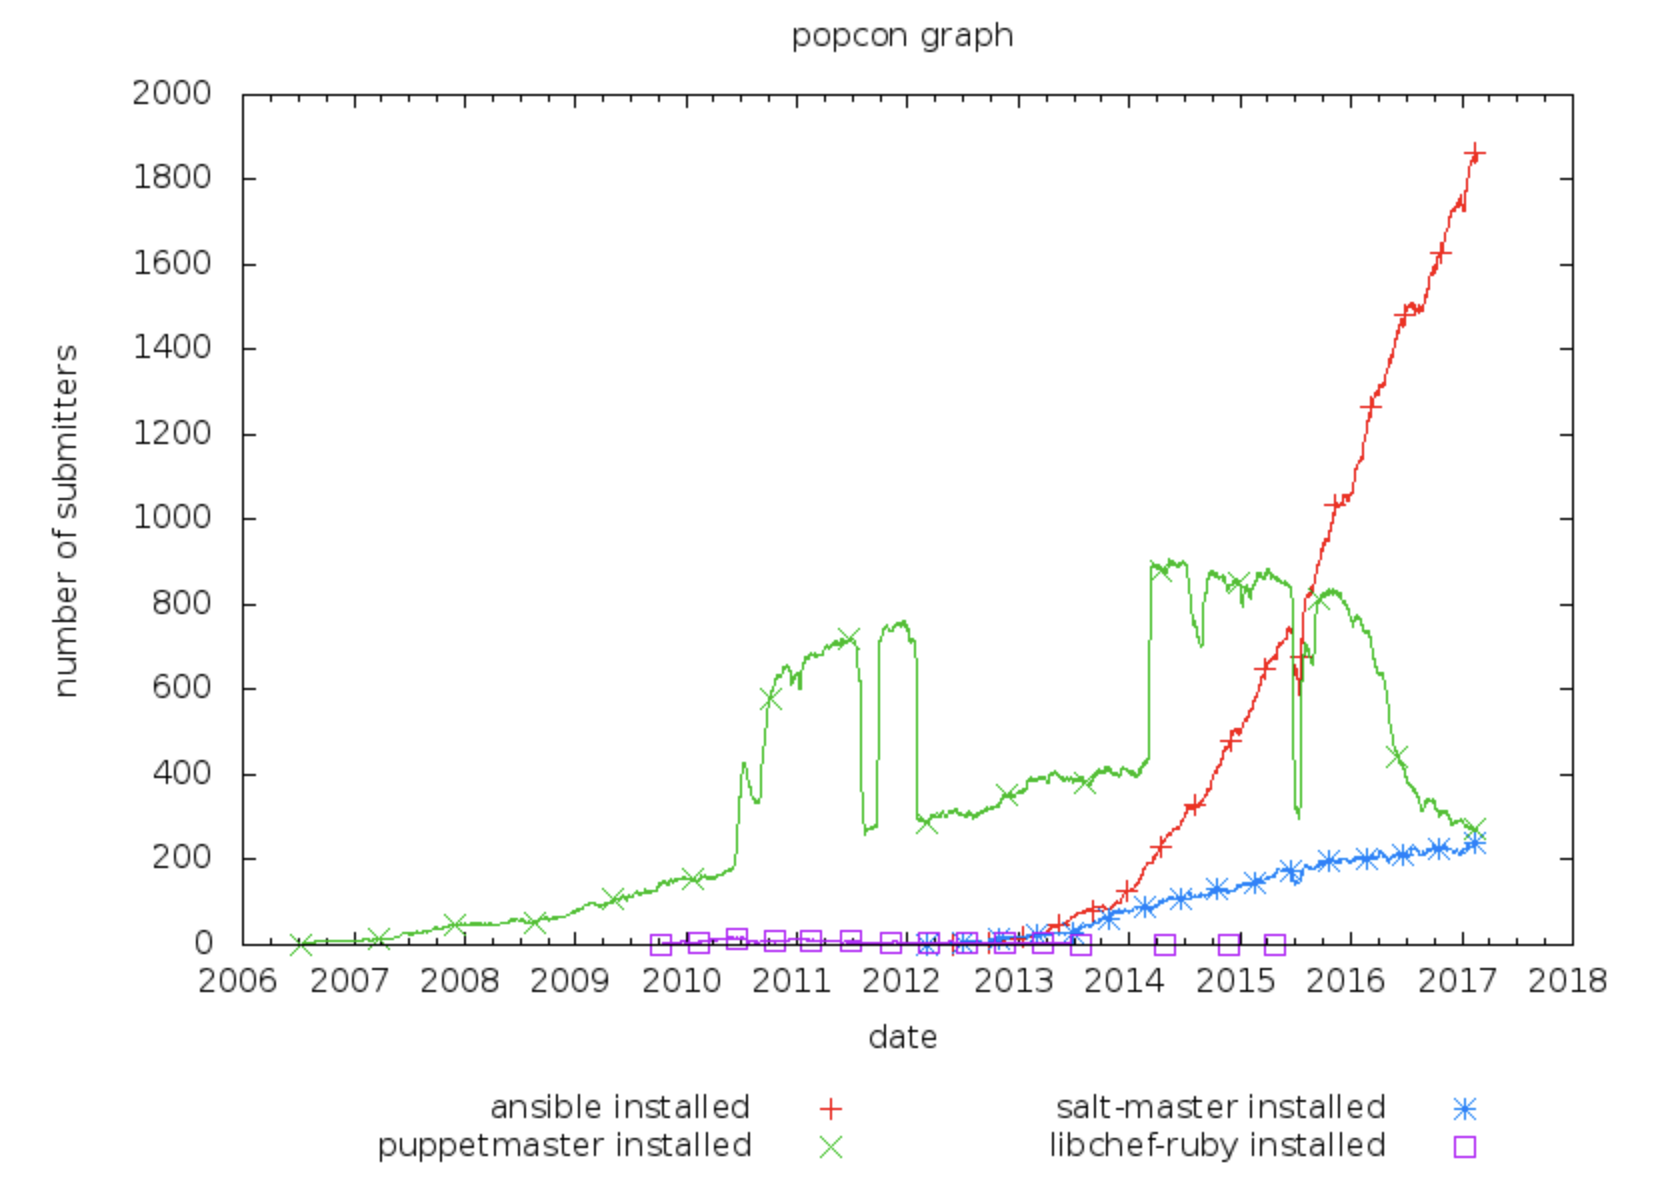
\includegraphics[width=\linewidth]{img/popcon_everybody.png}
  \caption{Deze grafiek toont het aantal keer dat een bepaald softwarepakket ge\"{\i}nstalleerd is op een Debian distributie. \autocite{popcon}}
  \label{fig:popcon_everybody}
\end{figure}

\subsection{Profiel van Puppet}
Puppet is een open source CMT die werd ontwikkeld in 2005 door Luke Kanies \autocite{PuppetLeaders} met als doel om op een betrouwbare mannier datacenters te kunnen automatiseren en te controleren. Dit zou het hele proces van services installeren moeten versnellen om zo tijd te winnen\autocite{how-puppet-works}. Dit kan zowel gaan om Linux servers als Windows servers \autocite{PuppetForWindows}. Om dit te kunnen verwezenlijken maakt Puppet gebruik van  het server/client model. De server wordt in dit model de Puppetmaster genoemd. Dit kunnen er  \'e\'en of meerdere zijn.  De client wordt de Puppetagent genoemd. Zowel op de master als op de agent dient Puppet ge{\"\i}nstalleerd te zijn om te kunnen functioneren. \autocite{puppetdoc} \autocite{puppetfaq}


\subsection{Profiel van Ansible}
Michael DeHaan is iemand die zeer vertrouwd was met Puppet. In zijn ervaring vond hij dat mensen moeilijkheden ondervonden op gebied van eenvoud en automatisatie. Bovendien waren er bedrijven die verschillende tools combineerden. Daarom wou Michael DeHaan een CMT bouwen die zorgde voor een duidelijk configuratie beheer, eenvoudig deployen van nieuwe servers en als het nodig was de mogelijkheid boodt tot ad-hoc commando's. Met dit idee is hij samen met met Sa{\"\i}d Ziouani in 2012 het open source project Ansible gestart \cite{ansiblefordevops}. Ook Ansible werkt volgens dit server/client model. Opvallend is wel dat elke computer waarop Ansible draait in principe kan fungeren als server. In bedrijven zoals de VRT wordt er wel gekozen voor een centraal punt. Dit wordt dan Ansible Tower genoemd. In tegenstelling tot Puppet dient er bij Ansible geen addionele software ge\"installeerd te worden op de clients. Dit komt het principe van eenvoudig deployen  ten goede.




%% TODO: deze sectie (die je kan opsplitsen in verschillende secties) bevat je
%% literatuurstudie. Vergeet niet telkens je bronnen te vermelden!





\section{Opzet van deze bachelorproef}
\label{sec:opzet-bachelorproef}



De laatste jaren is er een opwaarste trend in de digitaliserening van de wereld. Imec deed een onderzoek naar hoe mensen deze digitale bronnen consumeren. Hieruit bleek dat televie niet langer de alleenheerser is en dat steeds meer programma's worden bekeken via site's en app's. Zo is de populariteit van de televiesie als favoriete nieuwsmedium  in 2016 gezakt met 3,3\% t.o.v. het jaar daarvoor wat resulteert in een 22,4\%. Dit terwijl de smartphone, computer en tablet gezamenlijk 29,7\% halen \autocite{digimeter}. Het is vanzelfsprekend dat het mediahuis VRT deze trend moet volgen.
Bovendien wordt er een geheel nieuw gebouw verwacht dewelke ook het datacenter zal herbergen. Zo komt de VRT voor complexe vraagstukken te staan zoals: "'Hoe groot moet dit datacenter worden?"'  en "'Komen er extra locaties bij met back-up servers?"'.  Deze vragen moeten al een antwoord hebben voor de aanvang van het nieuwe gebouw. \newline

Al deze servers zijn van vitaal belang en zorgen voor een correcte werking van het mediabedrijf. Ze stockeren petabytes aan data en zijn verantwoordelijk voor een correcte uitzending van programma's. Veel afdelingen binnen de VRT maken bovendien gebruik van multi-stage omgevingen zoals testing, staging, productie... Het is dus belangrijk dat een geschikte CMT gebruikt wordt en dat deze perfect ge\"integreerd is met de bestaande en toekomstige infrastructuur.
In dit onderzoek vallen kleinere CMT's zoals Chef en Salt buiten de scope en zal de focus liggen op Puppet en Ansible. 
\newline
Dit onderzoek vindt plaats op MediaIT, een afdeling binnen de VRT zoals weerspiegeld is op het organigram in figuur \ref{fig:organigram}. Zij zijn \'e\'en van de afdelingen verantwoordelijk voor een goede en correcte werking van de servers. Zij gebruiken momenteel Puppet maar deze voldoet niet aan de verwachtingen van de bussiness. Zo is Puppet onder andere niet ge\"integreerd met de multi-stage omgevingen wat het testen bemoeilijkt. Verder is er een beperkte functionaliteit voor het monitoren van deploy's en daarom is er dan ook besloten om de huidige Puppet-infrastructuur te vervangen door Ansible.
\newline
Deze bachelorproef zal in deta\"il beschrijven en uitleggen wat er precies misgelopen is. Vervolgens zal er gekeken worden of Ansible deze problemen \"uberhaupt kan oplossen en hoe dit dan het beste gedaan wordt. Ook zal er een analyse gebeuren die de technische verschillen blootlegt.  Dit rapport wil een hulp bieden aan bedrijven die dezelfde stappen overwegen zodat het op voorhand duidelijk is wat er verwacht kan worden, wat de mogelijkheden zijn en waar een CMT te kort schiet. \newline
Ansible is sinds enige tijd aan een stevige opmars bezig maar er zijn voldoende voorbeelden van opensource (en andere) projecten die na een initi\"ele hype snel in mekaar zakten. Ondertussen heeft Ansible tal van mooie referenties achter zich en heeft het positieve analyses gekregen van belangrijke partijen zoals RedHat en Gartner. Is Ansible echter noemenswaardig beter dan bijvoorbeeld Puppet die reeds een lange bewezen staat van diens heeft (meer dan 12 jaar) en een grote community die het project ondersteunt?

\begin{figure}
  \begin{center}
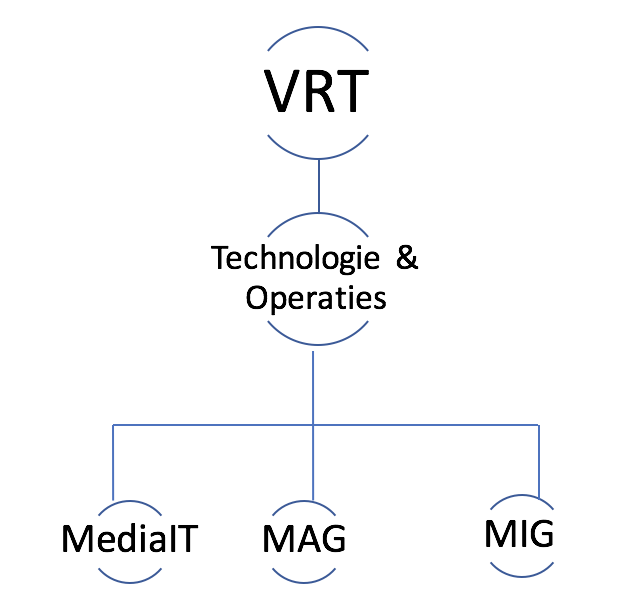
\includegraphics[width=100px]{img/organigram}
\end{center}  \caption{Organigram waarbinnen dit onderzoek zich afspeelt.}
  \label{fig:organigram}
\end{figure}

%%misschien staat dit beter bij opzet van bachelorproef.






\section{Probleemstelling en Onderzoeksvragen}
\label{sec:onderzoeksvragen}

%% TODO:
%% Uit je probleemstelling moet duidelijk zijn dat je onderzoek een meerwaarde
%% heeft voor een concrete doelgroep (bv. een bedrijf).
%%
%% Wees zo concreet mogelijk bij het formuleren van je
%% onderzoeksvra(a)g(en). Een onderzoeksvraag is trouwens iets waar nog
%% niemand op dit moment een antwoord heeft (voor zover je kan nagaan).


%% TODO: Het is gebruikelijk aan het einde van de inleiding een overzicht te
%% geven van de opbouw van de rest van de tekst. Deze sectie bevat al een aanzet
%% die je kan aanvullen/aanpassen in functie van je eigen tekst.

De overschakeling van Puppet naar Ansible is geen kleine stap en kan mogelijk voor veel complicaties zorgen. Daarom weet men best op voorhand wat er te wachten staat en zullen er in dit onderzoek verschillende relevante zaken onderzocht worden die kunnen worden opgedeeld in de volgende drie grote categorie\"en. 


\subsection{Wat zijn de redenen van een omschakeling?}

Het is belangrijk te weten wat de drijfveren waren voor de beslissing om Puppet te vervangen door Ansible en dat is precies waar deze eerste categorie toe dient. Om een profiel van de situatie op te kunnen stellen zal een interview plaatsvinden met de verantwoordelijken binnen de VRT om zo te achterhalen waar Puppet te kort schoot en waarom men denkt dat Ansible hier een oplossing biedt. Als bedrijven hun situatie herkennen in dit profiel, is het geadviseerd om te overwegen of een overstap ook voor hen al dan niet aan te raden is.

\subsection{Wat zijn de technische voor-en nadelen van Puppet en Ansible?}

In deze tweede categorie zal er een vergelijkende studie plaatsvinden waarbij technische aspecten zoals performantie, schaalbaarheid en veiligheid vergeleken worden. 
 
 Ten eerste wordt de performantie onderzocht. Hieronder wordt verstaan de tijd die nodig is tot het bekomen van een consistente staat en deze zal onderzocht worden in twee situaties. Bij de eerste is er namelijk nog geen configuratie aanwezig en dient alles nog ge\"installeerd en geconfigureerd te worden. Bij de tweede situatie is er wel al een configuratie aanwezig en is het de bedoeling dat de CMT enkel de nodige aanpassingen doorvoert en niet alles opnieuw configureert. 

Ten tweede is er de schaalbaarheid. Onder schaalbaarheid wordt verstaan: het vermogen om grote vraag te verwerken zonder kwaliteit te verliezen \autocite{informit}. We zullen monitoren hoe Ansible en Puppet hun resources verdelen bij een toenemende drukte, hier onder de vorm van meer servers en uitgebreidere configuraties. 

Er wordt afgesloten met een analyse over de veiligheid. Hierbij zal er een literatuurstudie plaatsvinden met onderzoek naar welke veiligheidsproblemen reeds gekend zijn en wat de impact hiervan is op een bedrijfsnetwerk. CMT's hebben namelijk  administrator rechten tot verschillende servers die ze dienen te configureren. Wanneer de server waarop een CMT draait besmet is, kunnen de gevolgen catastrofaal zijn.

\subsection{Wat is het verloop van een dergelijke transitperiode?}

Problemen die bij de vervanging van Puppet door Ansible optreden, zullen gerapporteerd worden en er zal onderzocht worden waarom deze optraden. Al dan niet gevonden oplossingen zullen beschreven en uitgelegd worden zodat andere bedrijven zich goed bewust zijn van wat er te wachten staat en hoe ze eventueel sommige voorvallen best kunnen oplossen. Welke incidenten zich zullen voordoen, valt uiteraard moeilijk te voorspellen. 

%%In Hoofdstuk~\ref{ch:methodologie} wordt de methodologie toegelicht en worden de gebruikte onderzoekstechnieken besproken om een antwoord te kunnen formuleren op de onderzoeksvragen.

%% TODO: Vul hier aan voor je eigen hoofstukken, één of twee zinnen per hoofdstuk

%%In Hoofdstuk~\ref{ch:conclusie}, tenslotte, wordt de conclusie gegeven en een antwoord geformuleerd op de onderzoeksvragen. Daarbij wordt ook een aanzet gegeven voor toekomstig onderzoek binnen dit domein.


%%=============================================================================
%% Methodologie
%%=============================================================================

\chapter{Methodologie}
\label{ch:methodologie}

%% TODO: Hoe ben je te werk gegaan? Verdeel je onderzoek in grote fasen, en
%% licht in elke fase toe welke stappen je gevolgd hebt. Verantwoord waarom je
%% op deze manier te werk gegaan bent. Je moet kunnen aantonen dat je de best
%% mogelijke manier toegepast hebt om een antwoord te vinden op de
%% onderzoeksvraag.

\section{Wat zijn de redenen van een omschakeling?}
\label{sec:methodologie-redenen-omschakeling}

TO DO
- slechte monitoring
- slecht geautomatiseert 
- geen multi environment
- expert vertrokken
- gui veel werk en complex
- oorspronkelijk geen modules, refactor, in feite nu weer refactor
- updates zorgen voor compatiblieteistproblemen (denk ik)
- puppet client niet ouder dan puppet master maar omgekeerd denkik wel (op te zoeken)

\section{Technische werking van Ansible en Puppet?}
\label{sec:methodologie-technische-verschillen}

\subsection{Overzicht van Puppet en Ansible}

\begin{minipage}{15cm}
\begin{tabular}{ r |c c }
& \textbf{Ansible} & \textbf{Puppet} \\
  \hline	  		
Programmeerparadigma\footnote{synoniemen zijn ook programmeerstijl of programmeermodel, voorbeelden zijn object-geori\"onteerd, procedureel, imperatief..., \autocite{journalofinformation} }  & declaratief & declaratief  \\
   \hline
 Programmeertaal & YAML & eigen DSL  \\
     \hline
   Communicatieprotocol & SSH & HTTPS \\
   \hline
   open poorten\footnote{Dit zijn de minimale vereisten van open poorten. Voor sommige features dienen meer poorten open te staan. Bijvoorbeeld 443 voor Ansible Tower of 8140 op elke Puppetclient voor de puppet kick functionaliteit \autocite{puppetkick} }  & 22/tcp (client) & 8140/tcp (master)\\
  \end{tabular}
  \end{minipage}   



 \autocite{languagePuppet}\autocite{masterproef} \autocite{ansibledoc}

\subsection{Werking van Puppet}

Tussen de master en de client bestaat er een vertrouwensrelatie die onderhouden wordt door certificaten. Het is de Puppetmaster die verantwoordelijk is voor het verlenen van deze certificaten. Pas als deze in orde zijn kan Puppet  aan de configuraties van de clients beginnen. De code die je schrijft wordt een manifest genoemd. Wanneer een Puppetagent wil controleren of hij nog up-to-date is, zal hij een catalogus aanvragen bij de Puppetmaster. Een dergelijke catalogus is in feite een manifest dat de Puppetmaster compileert. Deze catalogus is bovendien uniek voor elke Puppetagent. Dit komt omdat er bij het compileren van het manifest naar de catalogus rekening gehouden wordt met diverse parameters zoals de functie van de server of de distributie van het besturingssysteem dat op die server draait \autocite{Puppetlanguagecatalog}. Eens de Puppetagent zijn persoonlijke catalogus ontvangen heeft, zal deze voor zichzelf controleren of er verschillen zijn tussen zijn huidige configuratie en de staat die beschreven staat in de catalogus. Indien er afwijkingen zijn, worden deze ook automatisch opgelost \autocite{Puppetdoc}.

\begin{figure}  \begin{center}
  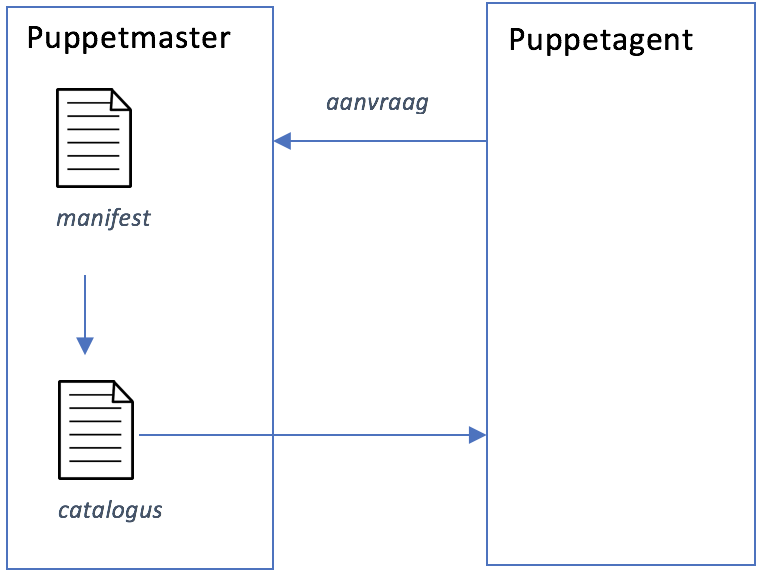
\includegraphics[width=250px]{img/aanvraagCatalogus.png}
 \end{center}\caption{aanvraag van een catalogus bij de Puppetmaster door een Puppetclient. De Puppetagent is een deamon (stukje software) die op de Puppetclient draait.}  
  \label{fig:aanvraagCatalogus}
\end{figure}


\subsection{Werking van Ansible}

Ansible maakt geen gebruik van agenten. Dit betekent dat de Ansibleserver enkel de naam en het wachtwoord dient te kennen van de servers die hij moet configureren. Het authenticeren kan op verschillende manieren. Er wordt aangeraden om gebruik te maken van een SSH-key, wat het eenvoudigst is, maar ook andere middelen zoals met een eenvoudig wachtwoord of het Kerberos-protocol worden ondersteund. De gewenste configuraties worden geschreven in playbooks met bijhorende modules. Eens een verbinding tot stand is gebracht wordt dit playbook met zijn modules verstuurd naar de te configureren server. Deze worden vervolgens op de Ansible clients uitgevoerd  en weer verwijderd. Ook Ansible bezit de functionaliteit om na te gaan of de huidige configuratie in lijn is met de ontvangen modules. Om servers te configureren met Ansible bestaan er bovendien twee manieren. Ansible playbooks kunnen in principe verstuurd worden naar de servers vanaf elke computer. Voor een grotere hoeveelheid servers is dit echter niet aangeraden en bestaat er de commerci"ele versie waarbij de playbooks worden verstuurd vanaf een centraal punt. Dit centraal punt is voorzien van Ansible Tower die een inventaris heeft van alle servers en playbooks die onder zijn verantwoordelijkheid vallen \autocite{ansibledoc}.


\subsection{Performantie}

Het is interessant om te weten wat de verhoudingen zijn tussen de deploy-tijd tussen Ansible en Puppet. Om dit op zo een betrouwbare mannier te kunnen verwezelijken zijn de configuraties van Ansible en Puppet zo analoog mogelijk gehouden en worden dus dezelfde services ge\"installeerd en geconfigureerd. Vervolgens wordt elke configuratie 30 keer uitgevoerd. De tijd kan worden onderverdeeld in twee delen.\newline
Het eerste deel van de tijd zal de connectietijd genoemd worden. Dit is de tijd die het kost totdat er effectief overgegaan kan worden tot configureren. Hieronder zitten zaken zoals het opstellen van een verbinding, het verzamelen van nodige gegevens en het versturen van een gepersonaliseerde configuratie. Bij Ansible kon deze tijd gewoon berekend\footnote{connectietijd = totaal verstreken tijd -  \unexpanded{$ \sum  $} (tijd playbooks)} worden op basis van de resultaten. Bij Puppet is dit echter niet mogelijk en bijgevolg zijn deze resultaten met de hand gemeten.\newline
 De tweede tijd is de tijd die nodig is om de configuratie effectief uit te voeren. Beide waarden zijn gebasseerd op de feedback van de corresponderende CMT.

\textbf{Tijd tot het bekomen van een verbinding (connectietijd)} (in seconden) \newline
\begin{tabular}{| r |c |c |c |c |c |c |c |c |c |c |c |c |c |c |c |c |c |c |c |c |c |c |c |c |c |c |c |c |c |c |c |c |c |c |}
  \hline	  		
Puppet & 9 & 6 & 6 & 11 & 6 & 7 & 8 & 6 & 9 & 9 & 7 & 7 & 8 & 6 & 6   \\ 
\hline
& 9 & 10 & 8 & 8 & 7 & 10 & 8 & 6 & 5 & 5 & 5 & 5 & 7 & 6 & 15\\
   \hline    \hline
  Ansible & 9 & 5 & 5 & 7 & 4 & 5 & 6 & 5 & 4 & 11 & 6 & 4 & 8 & 10 & 7 \\ 
\hline
   & 5 & 6 & 4 & 9 & 5 & 11 & 13 & 13 & 8 & 12 & 8 &	7 & 7 & 8  & 10 \\
  \hline  
\end{tabular}


\textbf{Tijd tot het bekomen van een consistente staat (deploytijd)} (in seconden)

\begin{tabular}{| r |c |c |c |c |c |c |c |c |c |c |c |c |c |c |c |c |c |c |c |c | c c |}
  \hline			
  
Puppet & 51,35 & 43,56 & 46,78 & 55,18 & 40,59 & 47,01 & 35,99 & 35,07 & 43,29 & 42,28  \\ \hline
           & 42,20 & 96,83 & 32,33 & 49,99 & 40,32 & 55,62 & 52,82 & 42,72 & 44,21 & 43,13 \\ \hline
            & 47,43 & 56,98	& 59,97 & 61,28 & 53,98	& 56,56 & 53,57 & 49,01 & 50,21 & 51,30 \\ \hline
              \hline 
   
  Ansible & 67 & 60 & 51 & 59 & 51 & 51 & 59 & 57 & 45 & 90 \\ \hline
                & 52  & 53 & 54 & 52 & 62 & 68 & 51 & 59 & 53 & 45  \\ \hline
                & 96 & 73 & 61 & 62	& 59 & 64	& 65 & 64 & 76 & 61  \\ \hline
                
  \hline  
\end{tabular}


\subsubsection{Deploytijd}
\begin{figure}
  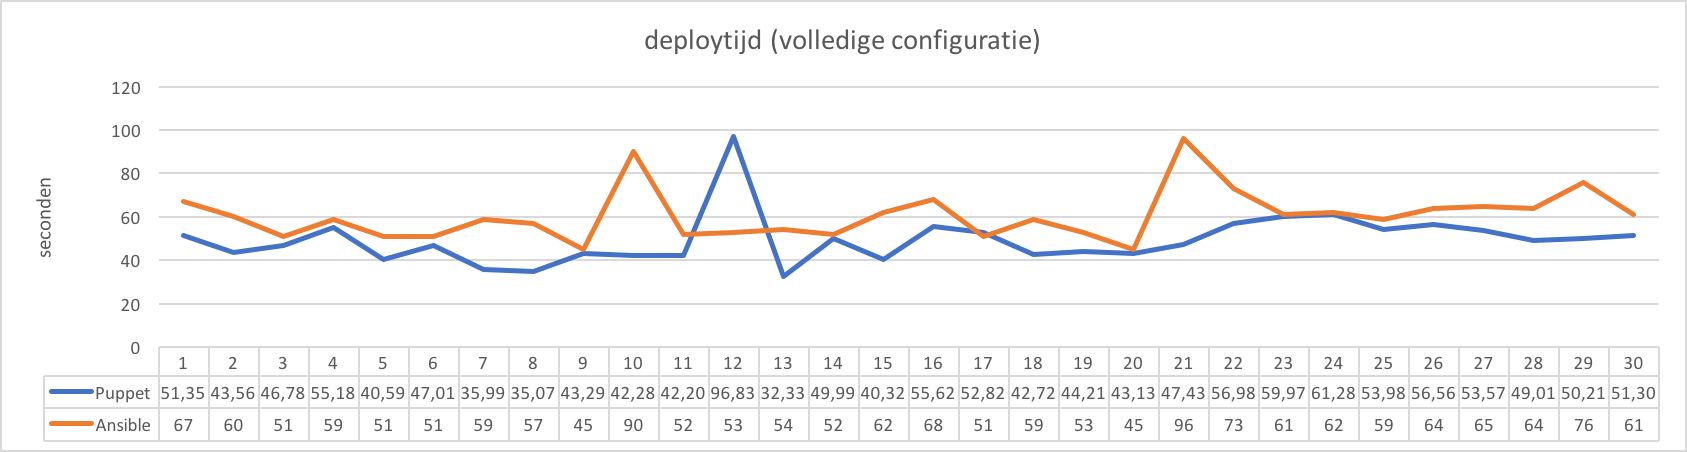
\includegraphics[width=\linewidth]{img/deploytime_fullconfig.png} 
  \caption{Tijd tot het bekomen van een consistente staat, vertrekende van een 'lege' server.}  
  \label{fig:deploytime_fullconfig}
\end{figure}

Aangezien grafiek \ref{fig:deploytime_fullconfig} geen duidelijk verschil toont tussen beide CMT's zal met behulp van de Z-toets aangetoond worden of er al dan niet een statistisch verschil is.

\underline{Hypothese}
\begin{align*}
H_0:  \mu_p = \mu_a \\
H_a: \mu_p\neq \mu_a 
\end{align*}


\underline{Significantieniveau en waarden} \newline

 $\alpha$ = 0.05 => -1.96 en +1.96 \newline

		\begin{tabular}{ r |c |c }
			& Puppet & Ansible\\\hline
			\unexpanded{$ \bar x  $} &  60.7 & 49.4\\ \hline
			$\sigma$ & 11.5 & 11.6\\ \hline
			n &  30 &  30

\end{tabular}


\underline{Toetsingsgrootheiden}
\begin{equation} \label{eq1}
\begin{split}
Z &= \tfrac{\bar x_p - \bar x_a}{\sqrt{\tfrac{\sigma_p^2}{n_p}+\tfrac{\sigma_a^2}{n_a}}}\\
& = \tfrac{49,4 - 60,7}{\sqrt{\tfrac{11,6^2}{30}+\tfrac{11,5^2}{30}}} \\
& = -3,789
\end{split}
\end{equation}



\underline{Conclusie} \newline
Z valt buiten het kritisch gebied waardoor de nulhypotese verworpen kan worden. Bijgevolg wordt aangenomen dat beide gemiddelde niet tot dezelfde verzameling behoren. Er kan dus worden geconcludeerd dat wanneer er wordt vertrokken van een lege server, Ansible er gemiddeld langer over doet dan Puppet. Dit is in dit geval een verschil van 11,3 seconden. \newline

De verschillen worden echter nog groter wanneer de test gedaan wordt met een gedeeltelijke configuratie. Hiermee wordt bedoelt dat er is vertrokken van servers die reeds geconfigureerd zijn en slechts enkele aanpassingen moeten doorgevoerd worden. Deze aanpassingen zijn een service starten en de inhoud van de webpagina veranderen. De resultaten lopen niet door elkaar waardoor een Z-toets niet echt nodig is. Ansible deed gemiddeld 19,10 seconden voor de deploy met een vrij grote variatie van 33,40 seconden. Puppet haalde maar een vrij consistente 3,10 seconden met een variatie van 0,35. \newline

In laatste instantie is er gekeken naar de tijd die het zou kosten totdat de CMT vaststelt dat de server reeds volledig is geconfigureerd en dat geen aanpassingen nodig zijn. Hierbij resulteert Ansible op een gemiddelde van 18 seconden met opnieuw een vrij grote variatie van 18,25 seconden. Ook hier doet puppet het opnieuw beter waarbij Puppet er minder dan een seconde nodig heeft om vast te stellen dan dat geen aanpassingen nodig zijn. Uiteraard zijn al deze waarden afhankelijk van de configuratie maar ze geven wel een duidelijke indicatie van de verschillen tussen beide CMT's.

\textbf{Opmerking:} De connectietijd is niet meegerekend in deze metingen. Het omvat hier uitsluitend de deploy tijd.
\subsubsection{Connectietijd}
Ook hier lopen de resultaten door elkaar zoals te zien is op grafiek \ref{fig:connectiontime}, bovendien liggen de gemiddelden hier veel dichter bij elkaar. Om vast te stellen of er een significant verschil zal er opnieuw gebruik gemaakt worden van de Z toets.
\begin{figure}
  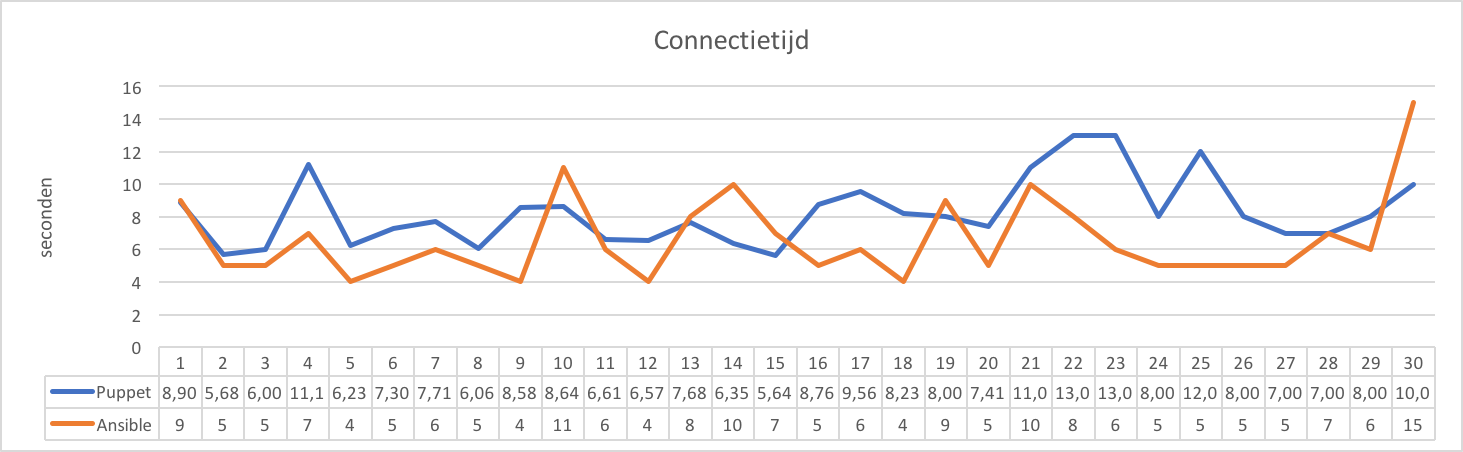
\includegraphics[width=\linewidth]{img/connectiontime.png} 
  \caption{Tijd tot het initialiseren van de deploy}  
  \label{fig:connectiontime}
\end{figure}



\underline{Hypothese}
\begin{align*}
H_0:  \mu_p = \mu_a \\
H_a: \mu_p\neq \mu_a 
\end{align*}
\underline{Significantieniveau en waarden} \newline

 $\alpha$ = 0.05 => -1.96 en +1.96 \newline

		\begin{tabular}{ r |c |c }
			& Puppet & Ansible\\\hline
			\unexpanded{$ \bar x  $} &  6,27 & 6,57\\ \hline
			$\sigma$ & 4,10 & 6,11\\ \hline
			n &  30 &  30

\end{tabular}


\underline{Toetsingsgrootheiden}
\begin{equation} \label{eq1}
\begin{split}
Z &= \tfrac{\bar x_p - \bar x_a}{\sqrt{\tfrac{\sigma_p^2}{n_p}+\tfrac{\sigma_a^2}{n_a}}}\\
& = \tfrac{ 6,27 - 6,57}{\sqrt{\tfrac{ 4,10 ^2}{30}+\tfrac{ 6,11^2}{30}}} \\
& = 1,27
\end{split}
\end{equation}
\underline{Conclusie}\newline
Z ligt in het aanvaardingsgebied waardoor we de nulhypothese, die stelt dat beide gemiddelden gelijk zijn, kunnen aanvaarden. Er is bijgevolg geen statistisch verschil tussen beide waarden.

%%---------------------------------------------------- einde performantie
\subsection{Belasting van het netwerk}

Ansible en Puppet hebben een groot verschil in de manier van communiceren en dit weerspiegeld zicht in het gedrag van de CMT. Op afbeelding \ref{fig:netwerkverbruikpernode} bevinden zich links alle Ansible clients, te herkennen aan hun naam die begint met een A. Rechts staan alle puppet clients, te herkennen aan de PP. De grafieken weerspiegelen uitsluitend het dataverkeer tussen de server (Ansible Tower of Puppetmaster) en de desbetreffende client. Andere data, zoals bijvoorbeeld het downloaden van services of uploaden van logbestanden naar de monitoringstool zijn hierin \underline{niet} opgenomen. Dit wordt verwezenlijkt door gebruik te maken van verschillende netwerkkaarten. Wanneer er geen deploy gebeurt is de kilobyte/ minuut op deze netwerkkaart gelijk aan nul, een bewijs dat hier geen andere data dan deze van de CMT over wordt verstuurd.  \newline

De mannier van communicatie is te herkennen in de grafieken. Zo onderhoud Ansible de communicatie met de client gedurende de deploy. Hiermee wordt bedoelt dat Ansible op de hoogte is van de laatste stand van zaken op de client. Wanneer een bepaalde taak voltooid is wordt Ansibel Tower hier onmiddelijk van op de hoogte gebracht. Zoals te zien is op de grafiek \ref{fig:deploytypes} is er geregeld communicatie tussen beide servers. Welliswaar is er enkel communicatie wanneer iets voltooid is, er is dus geen onnodige communicatie. Zo is ook te zien hoe op t6 de communicatie nul is. Ansible had voor die periode niets te melden\footnote{Hier betreft het de service MariaDB die werd ge\"installeerd}. \newline
 Deze mannier van werken is handig tijdens het schrijven van nieuwe Ansible rollen. Je krijgt namelijk live feedback tijdens het uittesten. Een nadeel hieraan is dat het netwerk geen rust krijgt. Bovendien word deze functionaliteit van 'live feedback' in productie niet vaak gebruikt. In realiteit lopen deze jobs tijdens de nacht en is het voldoende om de dag erop een algemeen overzicht te krijgen.\newline

Bij puppet is dit anders. Hierbij is er enkel communicatie tussen de server en de client op het begin en het einde van de deploy. Opmerkelijk hierbij is dat er twee types te herkennen zijn. Op figuur \ref{fig:deploytypes} zijn deze Puppet type A en B genoemd. Bij Puppet type A is te zien hoe de deploy bestaat uit twee reeksen terwijl dit bij type B uit drie reeksen bestaat. De oorzaak van deze derde reeks is niet gekend. Het opnieuw versturen van de tweede reeks was tijdelijk een piste maar dit is vermoedelijk niet het geval. Moest er een tcp-pakketje verloren gegaan zijn zou uitsluitend dat pakketje opnieuw verstuurd worden en niet de hele reeks. Verder heeft de poging om de inhoud van de pakketjes te lezen tot niet veel geleid. De verbinding is namelijk ge\"encrypteerd door het HTTPS-protocol met als gevolg dat tools zoals Wireshark of tcpdump geen oplossing konden bieden over de inhoud hiervan.\newline
Een nadeel aan het feit dat er enkel in het begin en het einde communicatie is, is dat er op de master geen live feedback voor testen gevolgd kan worden. Dit kan echter wel opgelost worden door in te loggen op de client en hier de live feedback volgen met het commando 'puppet agent -t'. Het wordt wel nog steeds pas op het einde van de deploy terug naar de master gestuurd?
 \newline


Vervolgens is er ook gekeken naar de totale netwerkbelasting. Hiervoor is er per client een cumulatie genomen van de kilobytes/minuut gedurende de gehele deploy. Deze waarden zijn terug te vinden in grafiek \ref{fig:netwerkverbruik}. Hier heeft Ansible een gemiddelde van 5802,29 kilobytes/deploy. Puppet heeft bij deploy's van type A (bestaande uit twee reeksen) een gemiddelde van  9392,5 kilobytes/deploy en bij type B (bestaande uit drie reeksen) 13742,35 kilobytes/deploy. Gezamenlijk heeft Puppet een gemiddelde van 11777,90 kilobytes/deploy. 


\begin{figure}
  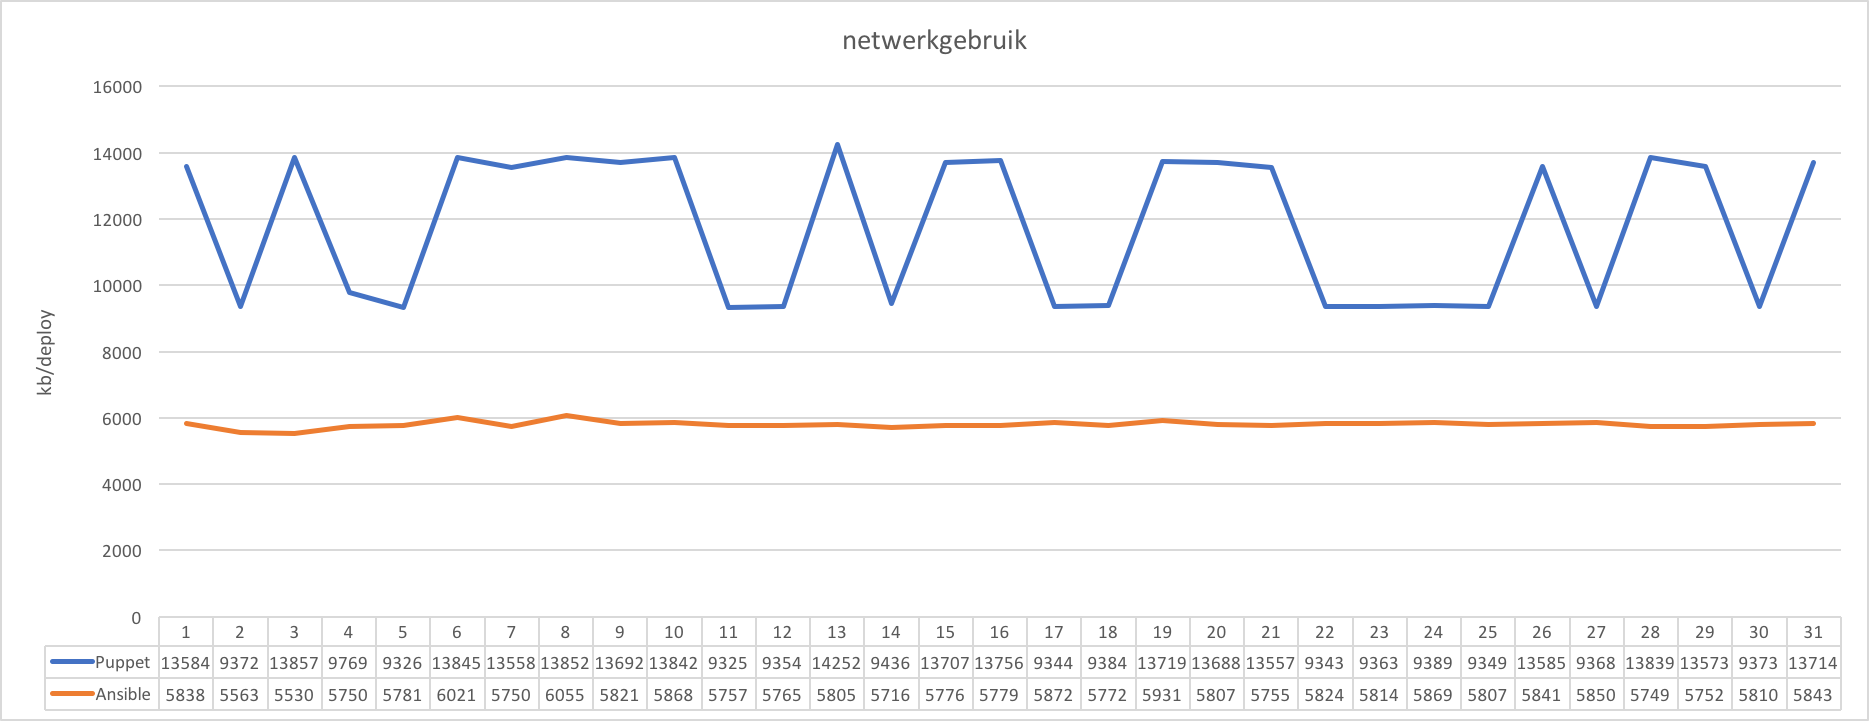
\includegraphics[width=\linewidth]{img/netwerkverbruik.png}
 \caption{Totaal verbruikte netwerkcapaciteit per client gedurende het deployen. Dit bevat enkel communicatie tussen master en client.}  
  \label{fig:netwerkverbruik}
\end{figure}


\begin{figure}
  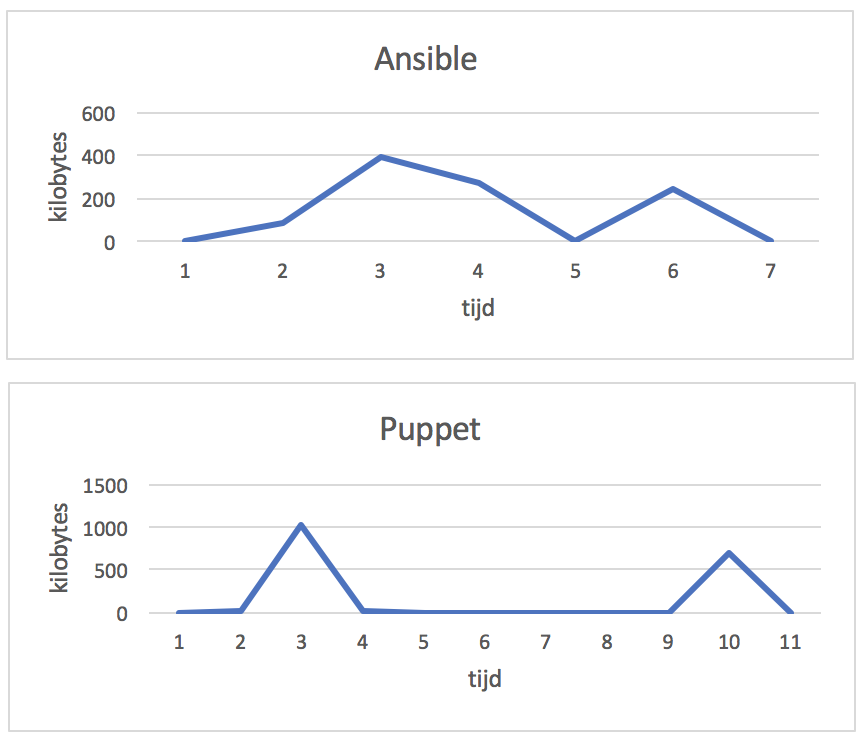
\includegraphics[width=\linewidth]{img/deploytypes.png}
 \caption{Drie types van communicatie. Aantal kilobytes per tijdseenheid op een netwerkkaart die uitsluitend bedoelt voor communicatie met Ansible Tower / Puppetmaster. }  
  \label{fig:deploytypes}
\end{figure}

\subsection{Gebruik van het geheugen}

Op grafiek \ref{fig:geheugengebruik} is per tijdseenheid het gemiddelde gebruikte ramgeheugen weergegeven. Hierop is te zien hoe Puppet opvallend meer geheugen gebruikt. Niet alleen tijdens een deploy maar ook ervoor en erna. Zelfs wanneer een Ansible client en een Puppet client juist opgezet worden met behulp van de Vagrantfile is er al een verschil in het gebruikte geheugen. Gezien het feit dat er al een verschil waar te nemen is in deze vroege levensfase van de server en het enige verschil in configuratie op dit moment de Puppetagent is werd vermoed dat het verschil hier aan te wijten is. Dit vermoeden werd gestaafd toen de Puppetagent tijdelijk uitgezet werd. Het ramgeheugen daalde onmiddelijk naar gelijkwaardige waarden als deze van de Ansibleclient. Zonder configuratie gebruiken Puppetclients gemiddeld 58\% geheugen van de 500MB ram. Bij Ansible is dit 47\%. Dit betekend dat met een verschil van 11\% er bij 500 MB, 55MB meer RAM-geheugen gebruikt wordt bij Puppet.


\begin{figure}
  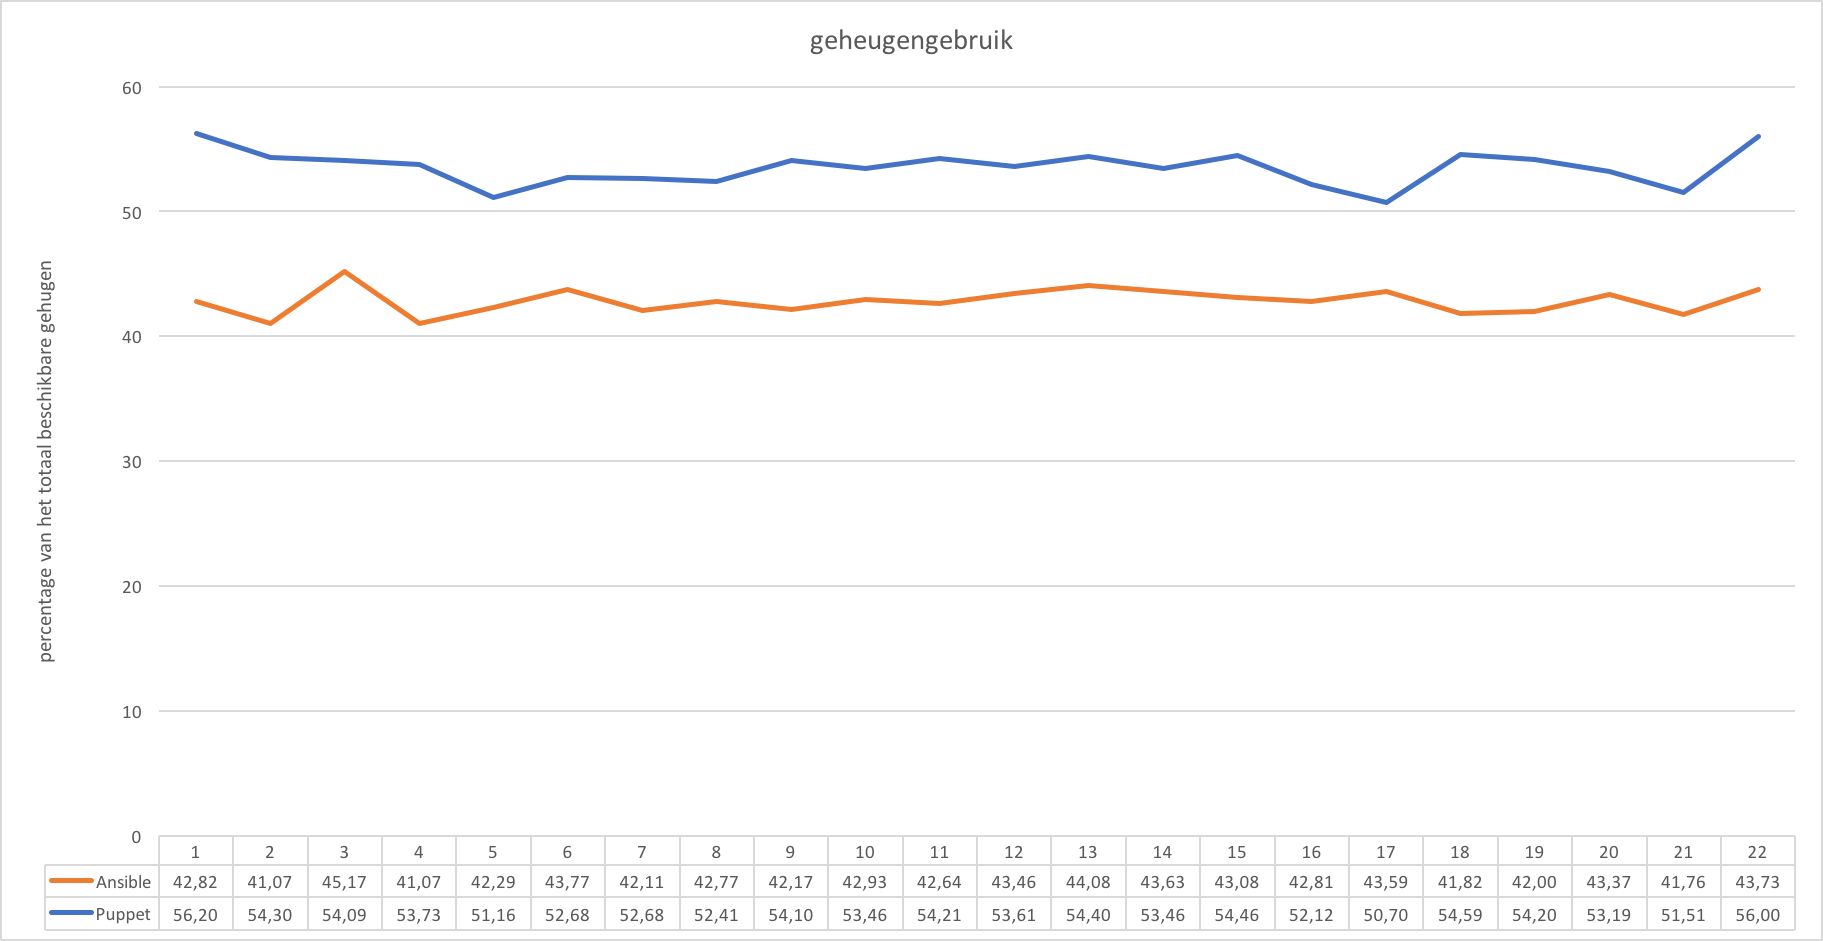
\includegraphics[width=\linewidth]{img/geheugengebruik}
 \caption{Verbruikt percentage van het RAM geheugen. Gemeten bij servers met elk 500 MB. }  
  \label{fig:geheugengebruik}
\end{figure}




\section{Wat is het verloop van een dergelijke transitperiode?}
\label{sec:methodologie-verloop-transit}











%% Voeg hier je eigen hoofdstukken toe die de ``corpus'' van je bachelorproef
%% vormen. De structuur en titels hangen af van je eigen onderzoek. Je kan bv.
%% elke fase in je onderzoek in een apart hoofdstuk bespreken.

%\input{}
%\input{}
%...

%%=============================================================================
%% Conclusie
%%=============================================================================

\chapter{Conclusie}
\label{ch:conclusie}

%% TODO: Trek een duidelijke conclusie, in de vorm van een antwoord op de
%% onderzoeksvra(a)g(en). Wat was jouw bijdrage aan het onderzoeksdomein en
%% hoe biedt dit meerwaarde aan het vakgebied/doelgroep? Reflecteer kritisch
%% over het resultaat. Had je deze uitkomst verwacht? Zijn er zaken die nog
%% niet duidelijk zijn? Heeft het ondezoek geleid tot nieuwe vragen die
%% uitnodigen tot verder onderzoek?

\lipsum[76-80]




%%---------  (eigen)-----------------------------
%%=============================================================================
%% Mathematiek
%%=============================================================================

\chapter{Bijlage A: Mathematische berekeningen}
\label{ch:mathematiek}

\section{Hypothese configuratietijd (volledige configuratie)}
\label{wis:hypothesedeploytijd}

Gebruikte dataset \ref{dataset:deploytijden}

\underline{Hypothese}
\begin{align*}
H_0:  \mu_p = \mu_a \\
H_a: \mu_p\neq \mu_a 
\end{align*}
\underline{Significantieniveau en waarden} \newline

 $\alpha$ = 0.05 => -1.96 en +1.96 \newline

		\begin{tabular}{ r |c |c }
			& Ansible & Puppet\\\hline
			\unexpanded{$ \bar x  $} &  60.7 & 49.4\\ \hline
			$\sigma$ & 11.5 & 11.6\\ \hline
			n &  30 &  30

\end{tabular}


\underline{Toetsingsgrootheden}
\begin{equation} \label{eq1}
\begin{split}
Z &= \tfrac{\bar x_p - \bar x_a}{\sqrt{\tfrac{\sigma_p^2}{n_p}+\tfrac{\sigma_a^2}{n_a}}}\\
& = \tfrac{49,4 - 60,7}{\sqrt{\tfrac{11,6^2}{30}+\tfrac{11,5^2}{30}}} \\
& = -3,789
\end{split}
\end{equation}

%-----------------------------------------------------------------------------------------------------------------
\section{Hypothese connectietijd}
\label{wis:hypotheseconnectietijd}

Gebruikte dataset \ref{dataset:deploytijden}

\underline{Hypothese}
\begin{align*}
H_0:  \mu_p = \mu_a \\
H_a: \mu_p\neq \mu_a 
\end{align*}
\underline{Significantieniveau en waarden} \newline

 $\alpha$ = 0.05 => -1.96 en +1.96 \newline

		\begin{tabular}{ r |c |c }
			& Puppet & Ansible\\\hline
			\unexpanded{$ \bar x  $} &  6,27 & 6,57\\ \hline
			$\sigma$ & 4,10 & 6,11\\ \hline
			n &  30 &  30

\end{tabular}


\underline{Toetsingsgrootheden}
\begin{equation} \label{eq1}
\begin{split}
Z &= \tfrac{\bar x_p - \bar x_a}{\sqrt{\tfrac{\sigma_p^2}{n_p}+\tfrac{\sigma_a^2}{n_a}}}\\
& = \tfrac{ 6,27 - 6,57}{\sqrt{\tfrac{ 4,10 ^2}{30}+\tfrac{ 6,11^2}{30}}} \\
& = 1,27
\end{split}
\end{equation}



%%---------- Samenvatting -----------------------------------------------------
%%
%% De samenvatting in de hoofdtaal van het document

\chapter*{Bijlage C: datasets}
\addcontentsline{toc}{chapter}{Bijlage C: datasets}


\section*{Netwerkverkeer}
\addcontentsline{toc}{section}{Netwerkverkeer}
\label{dataset:netwerkverkeer}
\subsection*{Netwerkverkeer: Puppet}
\addcontentsline{toc}{subsection}{Netwerkverkeer: Puppet}
\label{dataset:netwerkverkeer:puppet}
\begin{longtable}{ | l | l | l | l | l | l | l | l | l | l | l || l |  }

	\hline

	T1 & T2 & T3 & T4 & T5 & T6 & T7 & T8 & T9 & T10 & T11 & gemiddelde \\ \hline
	0 & 3270 & 1873 & 0 & 0 & 0 & 0 & 4259 & 0 & 0 & 0 & 9402 \\ \hline
	0 & 5115 & 0 & 0 & 0 & 0 & 0 & 0 & 4257 & 0 & 0 & 9372 \\ \hline
	0 & 5079 & 0 & 0 & 0 & 13 & 0 & 0 & 0 & 4280 & 0 & 9372 \\ \hline
	0 & 3248 & 2228 & 0 & 0 & 13 & 0 & 4280 & 0 & 0 & 0 & 9769 \\ \hline
	0 & 3203 & 1870 & 0 & 0 & 0 & 0 & 0 & 4253 & 0 & 0 & 9326 \\ \hline
	0 & 3202 & 1875 & 0 & 0 & 13 & 4278 & 0 & 0 & 0 & 0 & 9368 \\ \hline
	0 & 5102 & 0 & 0 & 0 & 0 & 4257 & 0 & 0 & 0 & 0 & 9359 \\ \hline
	0 & 5092 & 0 & 0 & 0 & 0 & 0 & 4265 & 0 & 0 & 0 & 9357 \\ \hline
	0 & 3222 & 1858 & 0 & 0 & 0 & 0 & 4261 & 0 & 0 & 0 & 9341 \\ \hline
	0 & 5063 & 0 & 0 & 0 & 0 & 0 & 4279 & 0 & 0 & 0 & 9342 \\ \hline
	0 & 5085 & 0 & 0 & 0 & 13 & 0 & 0 & 4227 & 0 & 0 & 9325 \\ \hline
	0 & 5080 & 0 & 0 & 0 & 13 & 0 & 4261 & 0 & 0 & 0 & 9354 \\ \hline
	0 & 5074 & 0 & 0 & 13 & 0 & 0 & 5156 & 0 & 0 & 0 & 10243 \\ \hline
	0 & 1641 & 3512 & 0 & 0 & 13 & 0 & 4270 & 0 & 0 & 0 & 9436 \\ \hline
	0 & 5084 & 0 & 0 & 0 & 13 & 0 & 4272 & 0 & 0 & 0 & 9369 \\ \hline
	0 & 5158 & 0 & 0 & 0 & 13 & 0 & 4248 & 0 & 0 & 0 & 9419 \\ \hline
	0 & 3210 & 1864 & 0 & 0 & 13 & 0 & 4257 & 0 & 0 & 0 & 9344 \\ \hline
	0 & 5086 & 0 & 0 & 13 & 0 & 0 & 4285 & 0 & 0 & 0 & 9384 \\ \hline
	0 & 5087 & 0 & 0 & 13 & 0 & 4281 & 0 & 0 & 0 & 0 & 9381 \\ \hline
	0 & 5059 & 0 & 0 & 13 & 0 & 4272 & 0 & 0 & 0 & 0 & 9344 \\ \hline
	0 & 5097 & 0 & 0 & 13 & 0 & 4247 & 0 & 0 & 0 & 0 & 9357 \\ \hline
	0 & 3011 & 2054 & 0 & 0 & 13 & 0 & 0 & 4265 & 0 & 0 & 9343 \\ \hline
	0 & 5077 & 0 & 0 & 13 & 0 & 0 & 0 & 4273 & 0 & 0 & 9363 \\ \hline
	0 & 5091 & 0 & 0 & 13 & 0 & 4285 & 0 & 0 & 0 & 0 & 9389 \\ \hline
	0 & 3210 & 1870 & 0 & 0 & 13 & 4256 & 0 & 0 & 0 & 0 & 9349 \\ \hline
	0 & 5092 & 0 & 0 & 13 & 0 & 0 & 5163 & 0 & 0 & 0 & 10268 \\ \hline
	0 & 5084 & 0 & 0 & 13 & 0 & 0 & 4271 & 0 & 0 & 0 & 9368 \\ \hline
	0 & 5076 & 0 & 0 & 13 & 0 & 4268 & 0 & 0 & 0 & 0 & 9357 \\ \hline
	0 & 5093 & 0 & 0 & 13 & 0 & 0 & 5134 & 0 & 0 & 0 & 10240 \\ \hline
	0 & 5072 & 0 & 0 & 13 & 0 & 0 & 0 & 4288 & 0 & 0 & 9373 \\ \hline
	0 & 5082 & 0 & 0 & 13 & 0 & 4285 & 0 & 0 & 0 & 0 & 9380 \\ \hline
\end{longtable}

\subsection*{Netwerkverkeer: Ansible}
\addcontentsline{toc}{subsection}{Netwerkverkeer: Ansible}
\label{dataset:netwerkverkeer:ansible}
\begin{longtable}{ | l | l | l | l | l | l | l | l | l | l | l || l | }

	\hline
	T1 & T2 & T3 & T4 & T5 & T6 & T7 & T8 & T9 & T10 & T11 & gemiddelde  \\ \hline
	0 & 1811 & 0 & 1133 & 1401 & 0 & 0 & 0 & 0 & 1071 & 422 & 5838  \\ \hline
	0 & 1838 & 0 & 2302 & 0 & 0 & 1371 & 52 & 0 & 0 & 0 & 5563    \\ \hline
	0 & 1832 & 0 & 2248 & 0 & 0 & 0 & 663 & 787 & 0 & 0 & 5530 \\ \hline
	0 & 1852 & 2153 & 316 & 0 & 0 & 0 & 1429 & 0 & 0 & 0 & 5750  \\ \hline
	0 & 1830 & 619 & 1877 & 0 & 0 & 1455 & 0 & 0 & 0 & 0 & 5781  \\ \hline
	0 & 1858 & 2713 & 0 & 0 & 762 & 688 & 0 & 0 & 0 & 0 & 6021   \\ \hline
	0 & 1830 & 490 & 1955 & 0 & 0 & 1428 & 47 & 0 & 0 & 0 & 5750  \\ \hline
	0 & 1824 & 0 & 2748 & 0 & 0 & 1431 & 52 & 0 & 0 & 0 & 6055   \\ \hline
	0 & 1855 & 168 & 2315 & 0 & 0 & 360 & 1123 & 0 & 0 & 0 & 5821  \\ \hline
	0 & 1826 & 168 & 2098 & 342 & 0 & 0 & 1434 & 0 & 0 & 0 & 5868  \\ \hline
	0 & 1859 & 1792 & 664 & 0 & 0 & 1442 & 0 & 0 & 0 & 0 & 5757 \\ \hline
	0 & 1865 & 0 & 2466 & 0 & 0 & 1375 & 59 & 0 & 0 & 0 & 5765  \\ \hline
	0 & 1846 & 168 & 2355 & 0 & 0 & 0 & 1436 & 0 & 0 & 0 & 5805 \\ \hline
	0 & 1819 & 498 & 1971 & 0 & 0 & 1428 & 0 & 0 & 0 & 0 & 5716   \\ \hline
	0 & 1852 & 2474 & 0 & 0 & 0 & 1450 & 0 & 0 & 0 & 0 & 5776   \\ \hline
	0 & 1832 & 168 & 2312 & 0 & 0 & 358 & 1109 & 0 & 0 & 0 & 5779  \\ \hline
	0 & 1852 & 0 & 930 & 1629 & 0 & 0 & 0 & 1461 & 0 & 0 & 5872    \\ \hline
	0 & 419 & 1452 & 909 & 1566 & 0 & 0 & 1426 & 0 & 0 & 0 & 5772  \\ \hline
	0 & 1865 & 0 & 883 & 1692 & 0 & 0 & 0 & 1109 & 382 & 0 & 5931   \\ \hline
	0 & 1879 & 0 & 2458 & 0 & 0 & 0 & 1048 & 422 & 0 & 0 & 5807 \\ \hline
	0 & 1826 & 2234 & 252 & 0 & 0 & 0 & 462 & 981 & 0 & 0 & 5755   \\ \hline
	0 & 1844 & 0 & 2530 & 0 & 0 & 0 & 1391 & 59 & 0 & 0 & 5824    \\ \hline
	0 & 1865 & 168 & 2317 & 0 & 0 & 0 & 1464 & 0 & 0 & 0 & 5814  \\ \hline
	0 & 1831 & 413 & 2096 & 0 & 0 & 0 & 1482 & 47 & 0 & 0 & 5869    \\ \hline
	0 & 1839 & 0 & 2484 & 0 & 0 & 0 & 1095 & 389 & 0 & 0 & 5807   \\ \hline
	0 & 1872 & 1444 & 1091 & 0 & 0 & 1434 & 0 & 0 & 0 & 0 & 5841 \\\hline
	0 & 1889 & 505 & 2031 & 0 & 0 & 0 & 0 & 1425 & 0 & 0 & 5850    \\ \hline
	0 & 1859 & 168 & 2293 & 0 & 0 & 1015 & 414 & 0 & 0 & 0 & 5749  \\ \hline
	0 & 1845 & 0 & 858 & 1599 & 0 & 0 & 796 & 654 & 0 & 0 & 5752   \\ \hline
	0 & 1862 & 0 & 2115 & 361 & 0 & 0 & 1070 & 402 & 0 & 0 & 5810   \\ \hline
	0 & 1845 & 534 & 1949 & 27 & 0 & 1070 & 418 & 0 & 0 & 0 & 5843   \\ \hline



\end{longtable}


\section*{ Geheugengebruik}
\label{dataset:geheugengebruik}
\addcontentsline{toc}{section}{Geheugengebruik}

\subsection*{Geheugengebruik: Puppet}
\addcontentsline{toc}{subsection}{Geheugengebruik: Puppet}
\label{dataset:deploytijden:puppet}

\begin{longtable}{ | l | l | l | l | l | l | l | l | l | l | l | l }
\hline
	38.02 & 48.85 & 64.39 & 58.46 & 67.23 & 68.15 & 63.54 & 57.98 & 39.22  & &  \\ \hline
	37.42 & 46.06 & 57.93 & 57.77 & 65.97 & 68.31 & 63.2 & 53.36 & 38.66 && \\ \hline
	37.70 & 42.26 & 57.95 & 55.13 & 66 & 67.53 & 67.56 & 62.64 & 45.18 & 38.93  & \\ \hline
	36.67 & 41.61 & 58.03 & 56.97 & 65.13 & 66.72 & 62.52 & 53.49 & 42.39 && \\ \hline
	36.99 & 41.3 & 48.8 & 57.57 & 65.01 & 67.31 & 63 & 51.31 & 41.55 & 38.71 & \\ \hline
	36.80 & 41.61 & 57.52 & 54.85 & 61.38 & 66.61 & 62.32 & 53.7 & 39.34 && \\ \hline
	38 & 48.7 & 61.46 & 60.96 & 66.70 & 62.36 & 54.25 & 42.47 & 39.19 && \\ \hline
	36.69 & 41.75 & 57.98 & 51.38 & 66.52 & 68.44 & 62.63 & 47.55 & 38.74 && \\ \hline
	37.33 & 45.9 & 64.3 & 57.66 & 67.31 & 67.22 & 53.91 & 39.16 &  && \\ \hline
	37.03 & 41.58 & 48.73 & 57.59 & 57.75 & 67.14 & 67.95 & 62.56 & 55.44 & 38.83 &    \\ \hline
	37 & 42.37 & 59.58 & 55.64 & 58.48 & 67.23 & 67.08 & 62.18 & 53.87 & 38.65 & \\ \hline
	37 & 41.61 & 57.97 & 54.09 & 66.49 & 68.04 & 66.36 & 51.82 & 39.09  & &\\ \hline
	37.03 & 48.05 & 64.32 & 57.52 & 67.27 & 68.38 & 62.5 & 45.87 & 38.66  & & \\ \hline
	36.69 & 41.63 & 57.97 & 55.94 & 65.91 & 67.98 & 68.05 & 58.06 & 43.89 & 38.49  & \\ \hline
	37.69 & 48.63 & 63.75 & 58.6 & 65.06 & 66.85 & 62.89 & 47.65 & 38.99&&    \\ \hline
	37.31 & 45.07 & 61.34 & 56.72 & 67.33 & 68.22 & 57.82 & 46.82 & 41.8 & 38.76  &  \\ \hline
	36.99 & 42.2 & 57.28 & 55.5 & 65.74 & 67.32 & 49.68 & 42.23 & 39.37   &&\\ \hline
	36.69 & 41.3 & 48.8 & 64.3 & 57.73 & 64.5 & 65.60 & 66.38 & 62.41 & 53.99 & 38.83  \\ \hline
	37.67 & 48.66 & 60.56 & 58.47 & 65.7 & 66.31 & 62.3 & 49.6 & 38.51&&  \\ \hline
	37.33 & 48.02 & 64.34 & 56.08 & 65.73 & 66.51 & 57.94 & 43.94 & 38.84 &&   \\ \hline
	36.89 & 44.85 & 57.86 & 48.88 & 66.55 & 68.41 & 57.49 & 44.51 & 38.18  && \\ \hline
	37.77 & 48.71 & 64.35 & 57.59 & 66.52 & 68.03 & 67.90 & 57.86 & 52.6 & 38.71 &  \\ \hline	
\end{longtable}

\subsection*{Geheugengebruik: Ansible}
\addcontentsline{toc}{subsection}{Geheugengebruik: Ansible}
\label{dataset:deploytijden:ansible}
\begin{longtable}{ | l | l | l | l | l | l | l | l | l | }
\hline
	28.45 & 46.62 & 38.17 & 50.78 & 49.33 & 40.54 & 31.5 &  &  \\ \hline
	28.48 & 33.23 & 40.31 & 41.26 & 50.89 & 49.7 & 40.63 & 31.49 &  \\ \hline
	29.17 & 46.64 & 44.1 & 50.83 & 52.12 & 32.17 &  &  &  \\ \hline
	28.41 & 31.28 & 46.75 & 44.14 & 50.86 & 49.93 & 32.9 & 31.6 &  \\ \hline
	28.44 & 41.05 & 39.67 & 50.74 & 50.82 & 48.81 & 33.43 & 31.51 &  \\ \hline
	28.69 & 46.71 & 41.26 & 50.8 & 48.44 & 31.66 &  &  &  \\ \hline
	28.42 & 31.46 & 38.67 & 49.11 & 50.86 & 52.09 & 41.17 & 31.43 &  \\ \hline
	28.43 & 34.86 & 39.87 & 50.74 & 50.85 & 48.82 & 31.49 &  &  \\ \hline
	28.42 & 38.58 & 37.19 & 34.72 & 50.79 & 53.09 & 49.02 & 31.82 &  \\ \hline
	28.41 & 33.97 & 38.63 & 49.6 & 50.86 & 55.29 & 40.42 & 31.72 &  \\ \hline
	28.14 & 42.31 & 36.57 & 41.56 & 50.33 & 54.77 & 41.76 & 31.21 &  \\ \hline
	27.77 & 30.66 & 45.93 & 40.55 & 50.22 & 50.24 & 50.27 & 48.3 & 31.49 \\ \hline
	27.8 & 40.44 & 37.76 & 50.21 & 50.25 & 51.82 & 46.83 & 31.22 &  \\ \hline
	27.84 & 40.54 & 46.02 & 35.36 & 50.27 & 50.29 & 54.06 & 41.29 & 31.21 \\ \hline
	27.84 & 29.36 & 46.03 & 43.23 & 50.35 & 52.6 & 48.49 & 31.52 &  \\ \hline
	27.82 & 33.44 & 47.45 & 38.56 & 50.27 & 50.3 & 48.29 & 31.38 &  \\ \hline
	27.82 & 40.76 & 34.26 & 50.26 & 52.57 & 51.02 & 32.66 &  &  \\ \hline
	28.15 & 41.08 & 34.30 & 50.27 & 52.62 & 41.39 & 31.26 &  &  \\ \hline
	27.84 & 30.76 & 46.02 & 43.56 & 50.32 & 51.91 & 40.24 & 31.21 &  \\ \hline
	27.83 & 37.97 & 40.13 & 45.08 & 50.32 & 50.28 & 48.38 & 31.46 &  \\ \hline
	28.09 & 42.83 & 35.52 & 50.24 & 50.32 & 48.39 & 32.78 & 32.22 &  \\ \hline
	27.9 & 40.79 & 40.65 & 50.3 & 50.35 & 50.89 & 41.84 & 31.27 &  \\ \hline
\end{longtable}




\section*{Deploytijden}
\addcontentsline{toc}{section}{Deploytijden}
\label{dataset:deploytijden}
\begin{longtable}{ | l | l || l | l || l | l || l | l | }
	\multicolumn{2}{c}{Connectietijd} & \multicolumn{2}{c}{\makecell*{Volledige\\configuratie}} &  \multicolumn{2}{c}{\makecell*{Gedeeltelijke\\configuratie}}  &   \multicolumn{2}{c}{\makecell*{Geen\\configuratie vereist}}  \\ \hline

	Puppet & Ansible & Puppet & Ansible & Ansible & Puppet &  Puppet &  Ansible \\ \hline
	8.9 & 9 & 51.35 & 67 & 14 & 2.92 & 0.41 & 19 \\ \hline
	5.68 & 5 & 43.56 & 60 & 20 & 3 & 0.38 & 11 \\ \hline
	6 & 5 & 46.78 & 51 & 23 & 2.96 & 0.34 & 12 \\ \hline
	11.18 & 7 & 40.59 & 59 & 23 & 2.98 & 0.37 & 18 \\ \hline
	6.23 & 4 & 55.18 & 51 & 14 & 2.91 & 0.39 & 22 \\ \hline
	7.3 & 5 & 47.01 & 51 & 19 & 5.86 & 0.38 & 20 \\ \hline
	7.71 & 6 & 35.99 & 59 & 30 & 3.11 & 0.4 & 9 \\ \hline
	6.06 & 5 & 35.07 & 57 & 15 & 2.93 & 0.43 & 11 \\ \hline
	8.58 & 4 & 43.29 & 45 & 21 & 2.88 & 0.42 & 16 \\ \hline
	8.64 & 11 & 42.28 & 90 & 22 & 3.24 & 0.38 & 10 \\ \hline
	6.61 & 6 & 42.2 & 52 & 14 & 3.19 & 0.62 & 11 \\ \hline
	6.57 & 4 & 96.83 & 53 & 14 & 4.36 & 0.36 & 10 \\ \hline
	7.68 & 8 & 32.33 & 54 & 20 & 2.95 & 0.38 & 15 \\ \hline
	6.35 & 10 & 49.99 & 52 & 25 & 2.93 & 0.36 & 17 \\ \hline
	5.64 & 7 & 40.32 & 62 & 13 & 2.97 & 0.36 & 19 \\ \hline
	8.76 & 5 & 55.62 & 68 & 14 & 2.9 & 0.4 & 15 \\ \hline
	9.56 & 6 & 52.82 & 51 & 13 & 2.96 & 0.35 & 22 \\ \hline
	8.23 & 4 & 42.72 & 59 & 18 & 2.85 & 0.42 & 16 \\ \hline
	8 & 9 & 44.21 & 53 & 16 & 2.95 & 0.59 & 16 \\ \hline
	7.41 & 5 & 43.13 & 45 & 24 & 2.87 & 0.39 & 19 \\ \hline
	11 & 10 & 47.43 & 96 & 19 & 2.87 & 0.4 & 19 \\ \hline
	13 & 8 & 56.98 & 73 & 15 & 2.87 & 0.38 & 19 \\ \hline
	13 & 6 & 59.97 & 61 & 23 & 3.09 & 0.42 & 10 \\ \hline
	8 & 5 & 61.28 & 62 & 13 & 2.95 & 0.44 & 9 \\ \hline
	12 & 5 & 53.98 & 59 & 14 & 2.93 & 0.44 & 10 \\ \hline
	8 & 5 & 56.56 & 64 & 32 & 2.96 & 0.4 & 11 \\ \hline
	7 & 5 & 53.57 & 65 & 14 & 2.93 & 0.9 & 10 \\ \hline
	7 & 7 & 49.01 & 64 & 14 & 2.88 & 0.42 & 11 \\ \hline
	8 & 6 & 50.21 & 76 & 25 & 2.8 & 0.42 & 11 \\ \hline
	10 & 15 & 51.3 & 61 & 32 & 3.1 &  & \  \\ \hline
\end{longtable}




%%-------------------------------- einde ruwe data




\chapter*{Lijst van woorden en afkortingen}

\begin{tabular}{l  l }
\textbf{Deploytijd} & De tijd die nodig is tot het bekomen van een consistente staat. \\ &Connectie tijd niet meegerekend. \\ \\
\textbf{Connetietijd} & De tijd die de CMT nodig heef totdat deze effectief over kan gaan tot configureren. \\ &  Hieronder vallen zaken zoals het maken van een verbinding, het verzamelen  \\ & van gegevens en opstellen van een gepersonaliseerde configuratie... \\ \\
\textbf{CMT} & Configuration management tool \\ \\
\textbf{fork} & Het aanmaken van een child process door zichzelf te dupliceren \autocite{forkmeaning} \\ \\
\textbf{Package manager} & Een mechanisme die het mogelijk maakt om software te installeren op UNIX gebaseerde systemen.\\ \textit{(voorbeelden: yum, apt, dpkg,...} \\
\end{tabular}


%%---------- Back matter ------------------------------------------------------
\printbibliography

\addcontentsline{toc}{chapter}{\textcolor{maincolor}{Bibliografie}}
%

\listoffigures
%\listoftables

\end{document}